% !TeX spellcheck = en_GB
% encoding: utf8
% !TEX encoding = utf8
% !TEX program = pdflatex
% !BIB program = biber

\documentclass[11pt,oneside,a4paper]{report}

\usepackage[utf8]{inputenc}
\usepackage[T1]{fontenc}
\usepackage[colorlinks]{hyperref}
\usepackage[left=2.5cm, right=2.5cm, top=2.5cm, bottom=2.5cm]{geometry}
\usepackage{float}
\usepackage{subcaption}
\usepackage{mathtools}
\usepackage{color}
\usepackage[backend=biber,maxnames=10,style=numeric,sorting=nty,abbreviate=false,giveninits=true,language=english]{biblatex}

\addbibresource{../meros.bib}

%\newcommand{\twc}[1]{\textcolor{red}{\textbf{TW}: #1}}
\newcommand{\Fig}[1]{Fig.~\ref{#1}}

\definecolor{amber}{rgb}{1.0, 0.49, 0.0}
\newcommand{\twci}[1]{
	\textcolor{amber}{TW: #1}}

% encoding: utf8
%
% Stereotypes
%

% Lista powinna być zgodna z profilem w EA

\newcommand{\stActionConn}{<<Action>>}
\newcommand{\stCommChannel}{<<CommChannel>>}
\newcommand{\stComponContain}{<<ComponContain>>}
\newcommand{\stGpPackages}{<<GpPackages>>}
\newcommand{\stHardware}{<<Hardware>>}
\newcommand{\stLaunchFile}{<<LaunchFile>>}
\newcommand{\stMetaPackage}{<<MetaPackage>>}
\newcommand{\stMicroNode}{<<MicroNode>>}
\newcommand{\stNamespace}{<<Namespace>>}
\newcommand{\stNode}{<<Node>>}
\newcommand{\stPackage}{<<Package>>}
\newcommand{\stParameter}{<<Parameter>>}
\newcommand{\stRepository}{<<Repository>>}
\newcommand{\stRosCommCompon}{<<RosCommCompon>>}
\newcommand{\stRosConn}{<<RosConn>>}
\newcommand{\stRQtNode}{<<RQtNode>>}
\newcommand{\stRunSystemCompon}{<<RunSystemCompon>>}
\newcommand{\stServiceConn}{<<Service>>}
\newcommand{\stSourExeContain}{<<SourExeContain>>}
\newcommand{\stSystem}{<<System>>}
\newcommand{\stTerminal}{<<Terminal>>}
\newcommand{\stTopicConn}{<<Topic>>}
\newcommand{\stWorkspace}{<<Workspace>>}

\newcommand{\stblock}{<<block>>}





\begin{document}
	
\title{MeROS: SysML-based Metamodel for ROS-related Systems - version 4.0.0 - reference manual}
\author{MeROS developers group - https://github.com/twiniars/MeROS \\ tomasz.winiarski@pw.edu.pl}
\date{\today}
\maketitle


\begin{abstract}
	The complexity of today's robot control systems implies difficulty in developing them efficiently and reliably. Systems engineering (SE) and frameworks come to help. The frameworks' metamodels are needed to support the standardisation and correctness of the created application models. MeROS is a~metamodel for ROS, which addresses the running system and developer workspace. An essential addition to the original ROS concepts is the grouping of these concepts, which provides an opportunity to illustrate the system's decomposition and varying degrees of detail in its presentation. The metamodel is derived from the requirements and verified on the practical examples. The matter is described in a~standardised way in SysML (Systems Modeling Language). Hence, common development tools that support SysML can help develop robot controllers in the spirit of SE.
\end{abstract}
	
	
	
	\maketitle
	
\chapter*{Important citation notice}

\textbf{If you are to use MeROS in your papers, please first cite the IEEE ACCESS  article~\cite{meros-access}, where the initial version of the MeROS is presented. You can also refer to MeROS project page \cite{meros-www} and mention the actual MeROS version you are using.}
	
	
\chapter{Introduction}
\label{ch:intro}	

	The development of civilisation has led to an increase in the importance of robotics. Many modern robotic systems are complex. To create them as effectively and reliably as possible, it is necessary to follow systems engineering (SE), where metamodels play an essential role~\cite{bezivin2004search,schmidt2006model,kent2002model}.
	Robots, especially complex ones, are mostly controlled with usage of software. Hence, in robotics, SE is inextricably linked with software engineering, where frameworks have been crucial for many years \cite{mnkandla2009software,shehory2014agent}.
	Diverse robotics frameworks have been developed so far \cite{inigo2012robotics,tsardoulias2017robotic,hentout2016survey}. Some steps towards standardisation have been made in recent years, and ROS (Robot Operating System) has come to the fore, currently in ROS~2 version \cite{maruyama2016exploring,park2020real}.   
	
	The robotic models can be subdivided~\cite{de2021survey} into Platform Independent Models (PIM), e.g., \cite{zielinski2017variable,zielinski2010motion,tasker2020,earl2020}, and Platform Specific Models (PSM). The metamodels of ROS, including MeROS, belong to PSM and should answer to the component nature of ROS \cite{Figat:2022:RAS,wenger2016model}.
	 MeROS is founded on SysML (Systems Modeling Language) \cite{omg-sysml17,Friedenthal:2015}, a~profile of UML (Unified Modeling Language). Modelling in languages from the UML family addresses a~number of important aspects of systems engineering \cite{chaudron2012effective}. These include the use cases [UCX]:
	\begin{itemize}
		\item $[$UC1] Systems' documentation and presentation,
		\item $[$UC2] Effective analysis of systems, especially in interdisciplinary teams (graphical language is more understandable for non-specialists in the field), 
		\item $[$UC3] Defects detection,
		\item $[$UC4] Integration of new collaborators into the development team,
		\item $[$UC5] Resuming work after a~break,
		\item $[$UC6] Extension and modification of existing systems,
		\item $[$UC7] Support the implementation of new systems,
		\item $[$UC8] Migration of systems.
	\end{itemize}
	
	In practice, documentation is created both prior to implementation and, in many cases, through a~process of reverse  engineering \cite{canfora2007new} for existing systems. Agile-type strategies involve modifying the documentation as the project develops \cite{habib2021systematic}. Systems development with V-model-based application of MeROS metamodel was proposed in \cite{winiarski2025-v-model}.
			
	The following presentation starts with formulating the requirements (chapter~\ref{ch:requirements}) for the MeROS metamodel. These requirements are allocated to the metamodel that's architecture is described in chapter~\ref{ch:metamodel}. The way to present a~model of a~specific application based on MeROS is presented on a~practical example in chapter~\ref{ch:application}.
	
	
\chapter{Metamodel requirements}
\label{ch:requirements}
	The requirements [RX] formulation process for MeROS metamodel is multi-stage and iterative. In the beginning, the initial requirements were formulated based on: (i) literature review (both scientific and ROS wiki/community sources), (ii) author experience from supervising and supporting ROS-related projects, and finally, (iii) author experience from EARL (Embodied Agent-based cybeR-physical control systems modelling Language) \cite{earl2020} PIM development and its applications (e.g. \cite{tasker2020,karwowski2021hubero,en14206693-grav-comp}). Verification of subsequent versions of MeROS by its practical applications led to an iterative reformulation of requirements and MeROS itself. 
	
	MeROS requirements are depicted on a~number of dedicated SysML diagrams. The requirements are organised in a~tree-like nesting structure, with additional internal relations, and labelled following this structure. The general requirements are presented in Fig.~\ref{fig:general_req}. 
		
	\begin{figure}[H]
		\centering
		\begin{center}
			{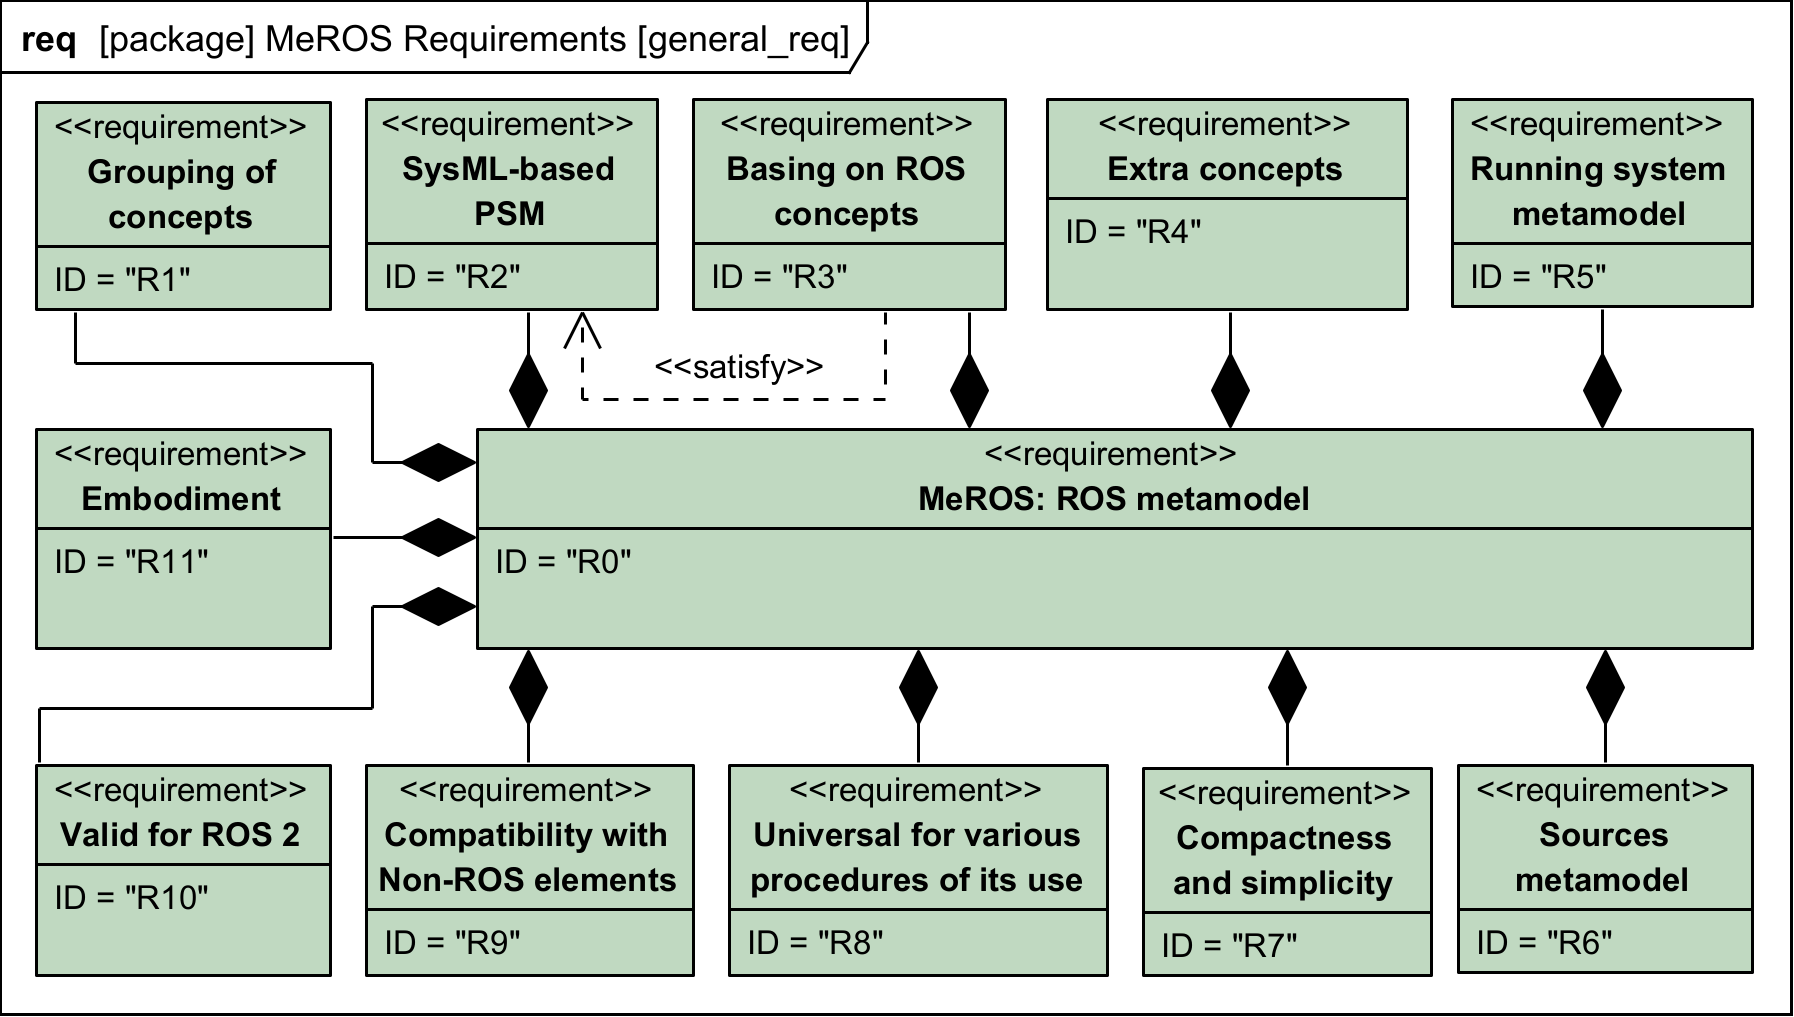
\includegraphics[scale=1.0]{diagrams/general_req.png}}
		\end{center}
		\caption{General requirements.} 
		\label{fig:general_req}
	\end{figure}
		
	The SysML models have two main parts: behavioural [R1] and structural [R2]. MeROS aims to cover ROS concepts [R3] and not change their labels as long as possible, to maintain conformity and intuitiveness. The ROS system is two-faced. While it is executed [R4], it has a~specific structure and behaviour, but from the developers' point of view, the sources [R5] are the exposed aspect. The model should be compact and straightforward [R6] rather than unnecessarily elaborate and complicated. It is also universal. It does not imply itself the specific procedure of its use [R7]. These procedures are specified outside of the MeROS metamodel. Although the SysML-based MeROS is classified into PSM [R8], it should be compatible with Non-ROS elements [R9]. MeROS metamodel should be valid for ROS~2 [R10]. Finally, embodiment [R11] (e.g. system deployment) should be considered.
	
	The system's structural aspects requirements are presented in Fig.~\ref{fig:structural_aspects_req}.
	
	\begin{figure}[H]
		\centering
		\begin{center}
			{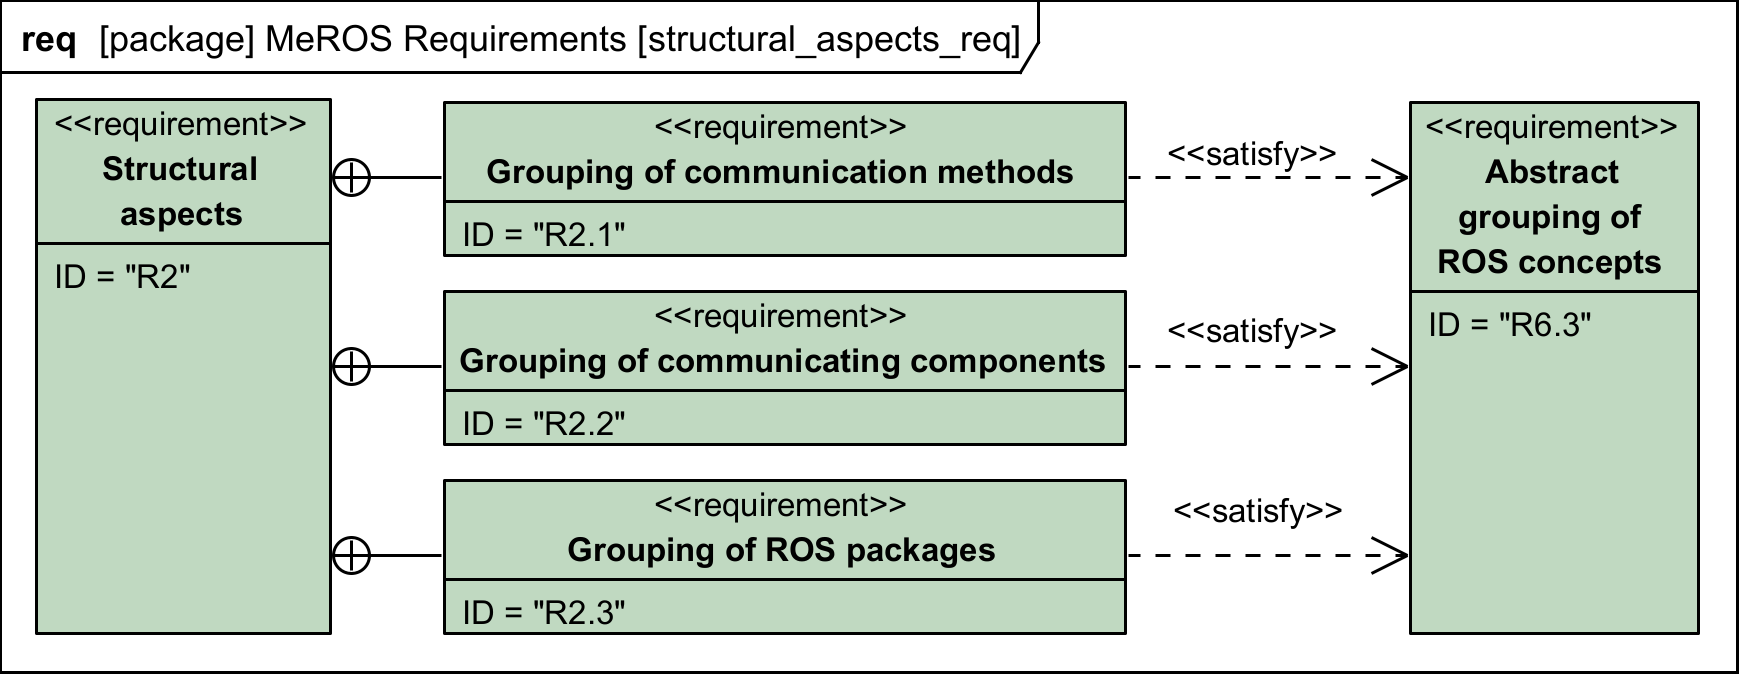
\includegraphics[scale=1.0]{diagrams/structural_aspects_req.png}}
		\end{center}
		\caption{Structural aspects requirements.  \twci{tutaj w ogóle jest kuriozum. Abstrakt grouping jest w nieintuicyjny sposób pod kompactenss i simliity. Tew grupowania to odrazu powinny być grupy i raczej dołączone do ogólnego wymagania na grupowania a nie aspektów strukturalnych}} 
		\label{fig:structural_aspects_req}
	\end{figure}
	
	A~vital addition to the original ROS concepts is the abstract grouping of: (i) communicating methods [R2.1] and (ii) communicating components [R2.2]. The motivation for the introduction of these aggregates is presented further on. It should be noted that several ROS concepts group other concepts in a~particular way, especially to deploy the system. Action aggregates Topics and Services (in ROS~2), ROS~1 Node aggregates Nodelets, and ROS~2 Component Container aggregates Nodes.
		
	The ROS concepts that MeROS models are organised into four major classes (Fig.~\ref{fig:ros_concepts_req}): (i)~Communicating components [R3.1], (ii) Communication methods [R3.2], (iii) Workspace [R3.3], and (iv) Other [R3.4].
	

	\begin{figure}[H]
		\centering
		\begin{center}
			{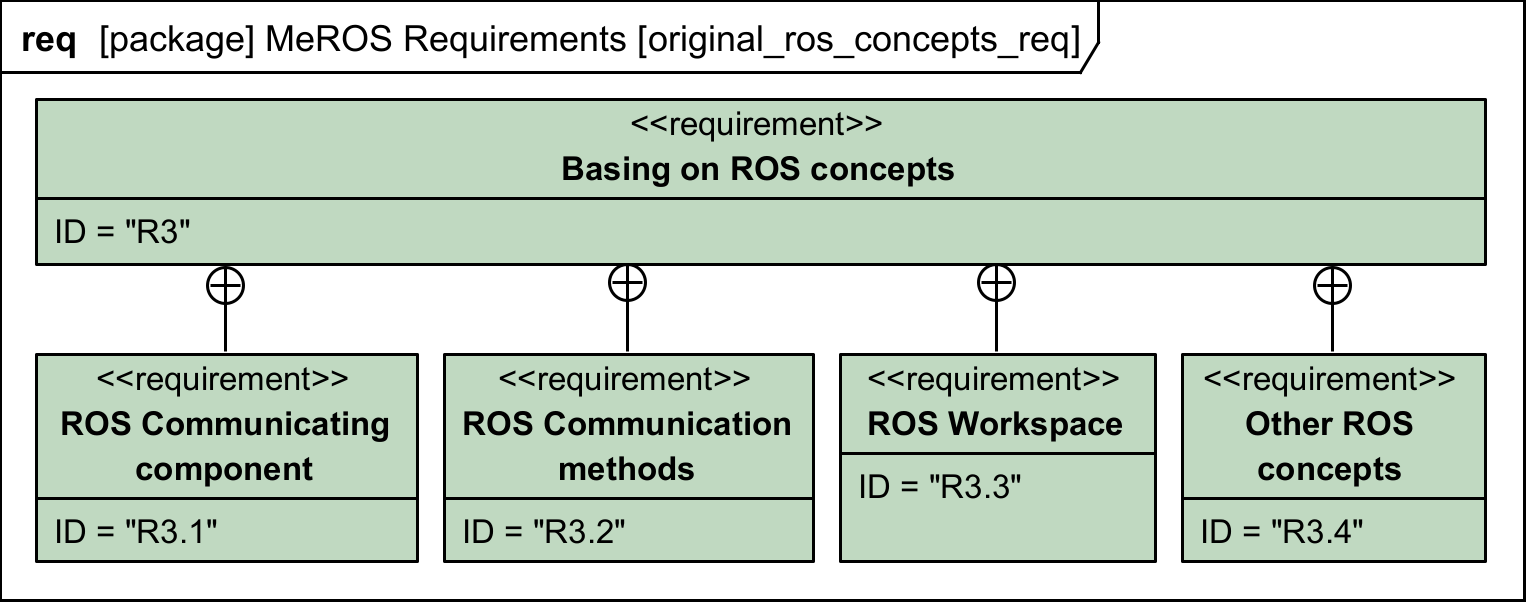
\includegraphics[scale=1.1]{diagrams/original_ros_concepts_req.png}}
		\end{center}
		\caption{ROS concepts requirements. \twci{tutaj w miejsce ros workspace powinno być ROS source containers}} 
		\label{fig:ros_concepts_req}
	\end{figure}
	 \twci{gałąź ros concepts powinna być konsekwetnie poprowadzona}
	\pagebreak
	
	ROS Communicating components [R3.1] are (Fig.~\ref{fig:communicating_components_req}): (i) ROS Node.

	\begin{figure}[H]
		\centering
		\begin{center}
			{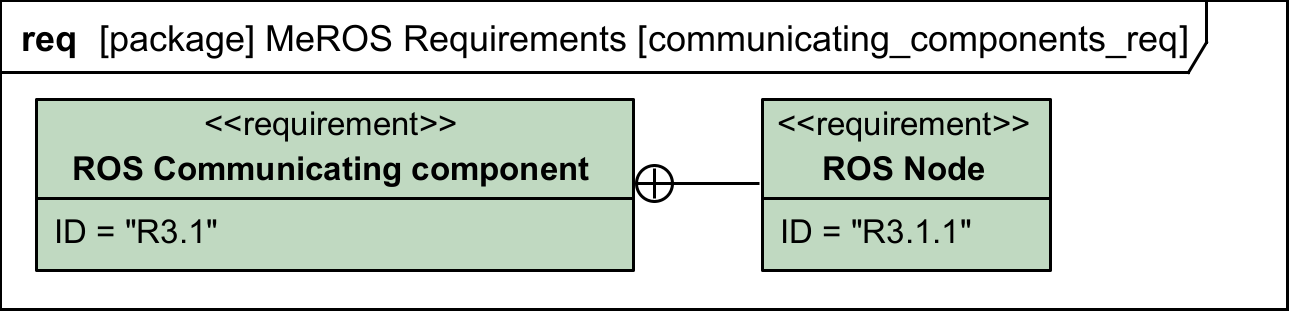
\includegraphics[scale=1.1]{diagrams/communicating_components_req.png}}
		\end{center}
		\caption{Communicating components requirements.} 
		\label{fig:communicating_components_req}
	\end{figure}
	
	Communication methods are depicted in Fig.~\ref{fig:communication_concepts_req}.
	 Three methods of communication are considered [R3.2] with their inter-component connections and data structures: (i) ROS Topic, its Message and connection, (ii) ROS Service comprising data structure and connection, and finally (iii) ROS Action including data structure and connection.
	
	\begin{figure}[H]
		\centering
		\begin{center}
			{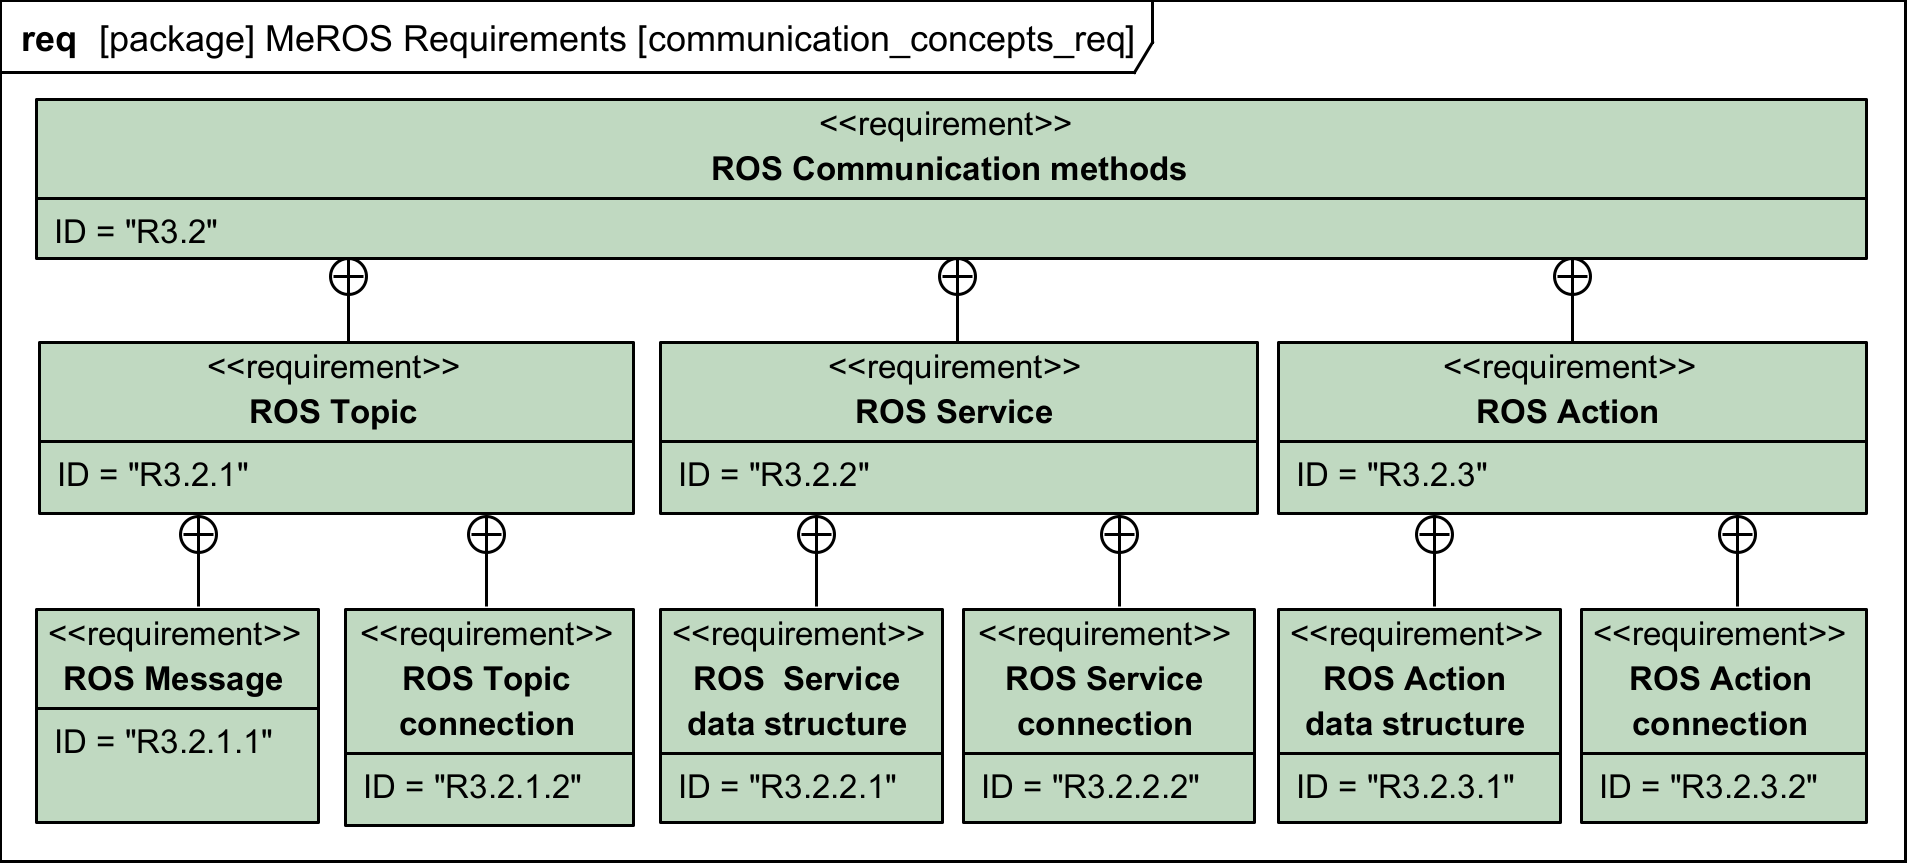
\includegraphics[scale=.98]{diagrams/communication_concepts_req.png}}
		\end{center}
		\caption{Communication concepts requirements.} 
		\label{fig:communication_concepts_req}
	\end{figure}
	
	Workspace concept [R3.3] comprises (Fig.~\ref{fig:workspace_concepts_req}): (i) ROS Package [R3.3.1], (ii) ROS Metapackage [R3.3.2] introduced in the latest releases of ROS~1, (iii) Group of ROS packages [R3.3.3], and (iv) Repository [R3.3.4]. In practise ROS Metapackage is a~specific, degenerated ROS Package.
	
	\begin{figure}[H]
		\centering
		\begin{center}
			{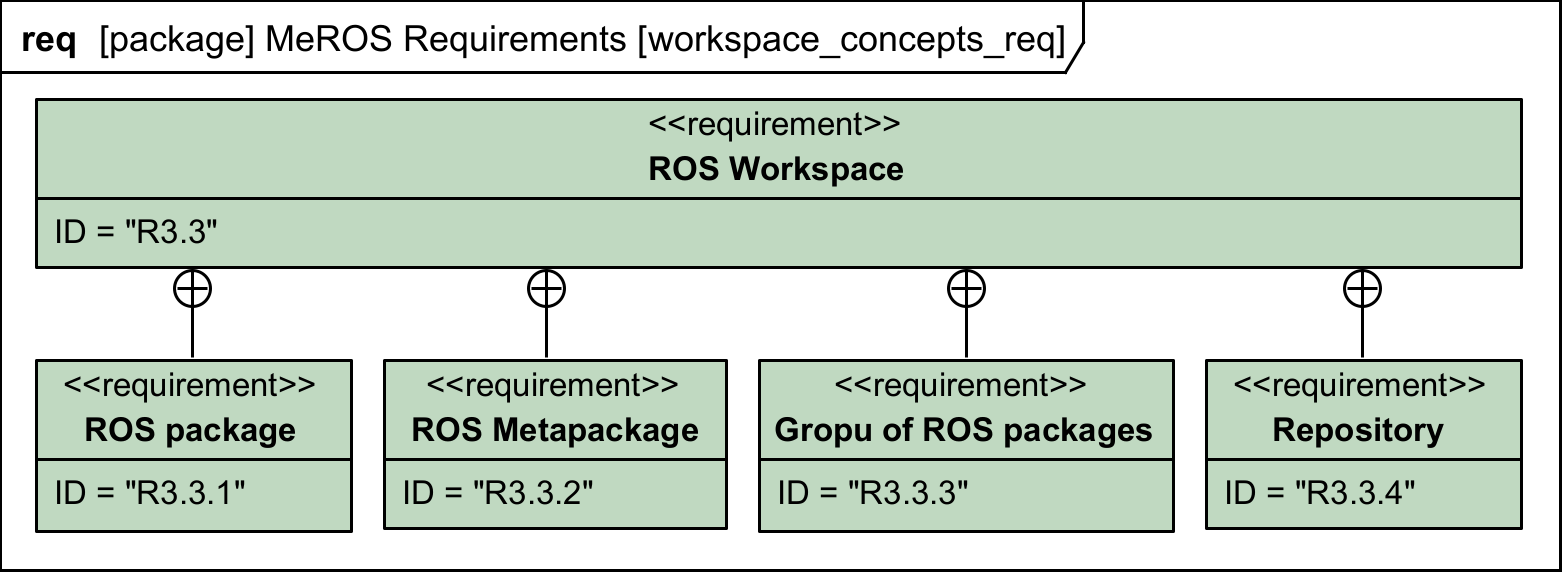
\includegraphics[scale=1.0]{diagrams/workspace_concepts_req.png}}
		\end{center}
		\caption{Workspace concepts requirements.} 
		\label{fig:workspace_concepts_req}
	\end{figure}
	
	\pagebreak
	
	Other concepts (Fig.~\ref{fig:other_concepts_req}) [R3.4] include two elements: (i) ROS Parameters, (ii) ROS Namespace reflects the ROS concept to organise nodes and communication connections.
	
	\begin{figure}[H]
			\centering
			\begin{center}
					{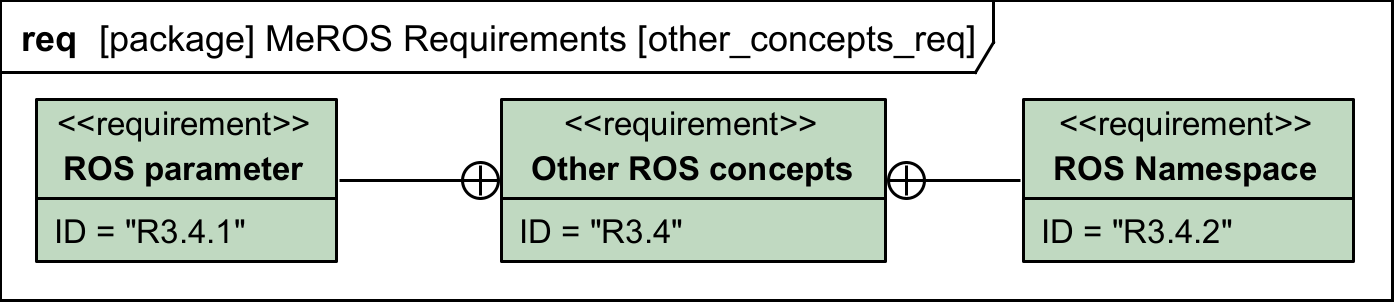
\includegraphics[scale=1.0]{diagrams/other_concepts_req.png}}
				\end{center}
			\caption{Other ROS concepts requirements.} 
			\label{fig:other_concepts_req}
		\end{figure}


	To achieve intuitiveness, MeROS presents a~Running system structure (Fig.~\ref{fig:running_system_req}) following ROS rqt\_graph pattern [R4.1]. In particular, there are two ways to visualise communication, including [R4.1.1] and without [R4.1.2]
	dedicated communication components.
	\begin{figure}[H]
		\centering
		\begin{center}
			{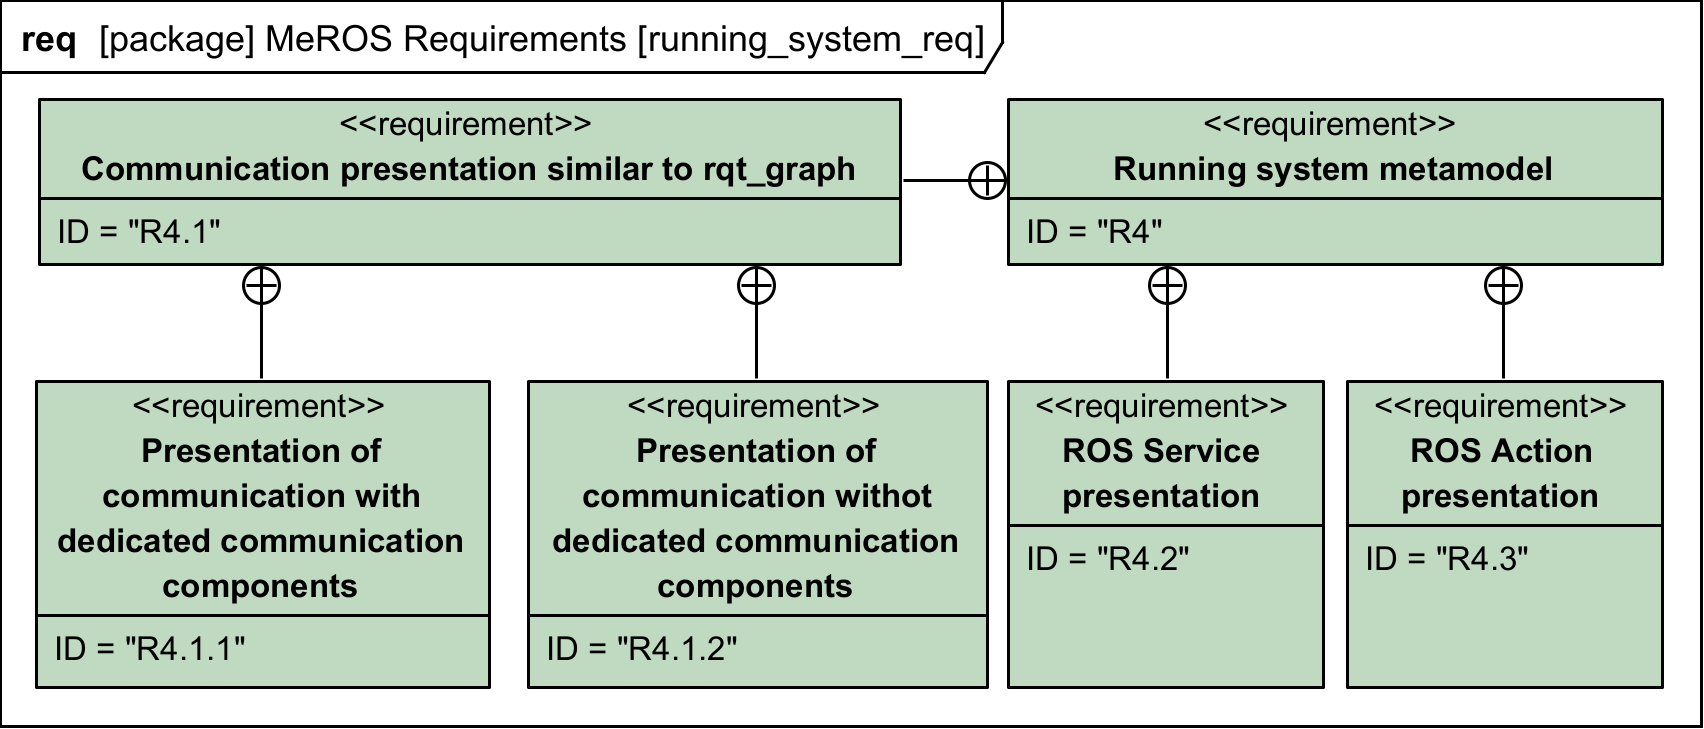
\includegraphics[scale=1.0]{diagrams/running_system_req.png}}
		\end{center}
		\caption{Running system requirements. \twci{Dlaczego nie ma ros topic presentation? Dlazego nei wuzględniono roznych metod prezetnacji akcji i serwisow? Dlaczego nei ma prezetancji wezłow?}} 
		\label{fig:running_system_req}
	\end{figure}
	 The dedicated components are especially useful in the presentation when many communication components use the same topic both on the publisher and the subscriber side. In opposition, the expression of topic names on arrows connecting communicating components, i.e., without dedicated communication components, let to reduce the number of components needed to depict communication for many topics and a~low number of communicating components. The other advantage of using dedicated communication components is that the particular connection can be split into several diagrams (e.g. ibd (internal block diagram) or sd (sequence diagram)), where the same object represents this connection in every associated diagram. Services [R4.2] and actions [R4.3] should be depicted as an addition to the presentation of the particular topics. It should be noted that rqt\_graph represents actions as a~number of topics and services. In MeROS, the topics and services being part of an action can be aggregated, which reduces the number of depicted connections.
		
	\pagebreak
			
	The compactness and simplicity [R6] and its nesting requirements are presented in Fig.~\ref{fig:compactness_and_simplicity_req}. 
	
	\begin{figure}[H]
		\centering
		\begin{center}
			{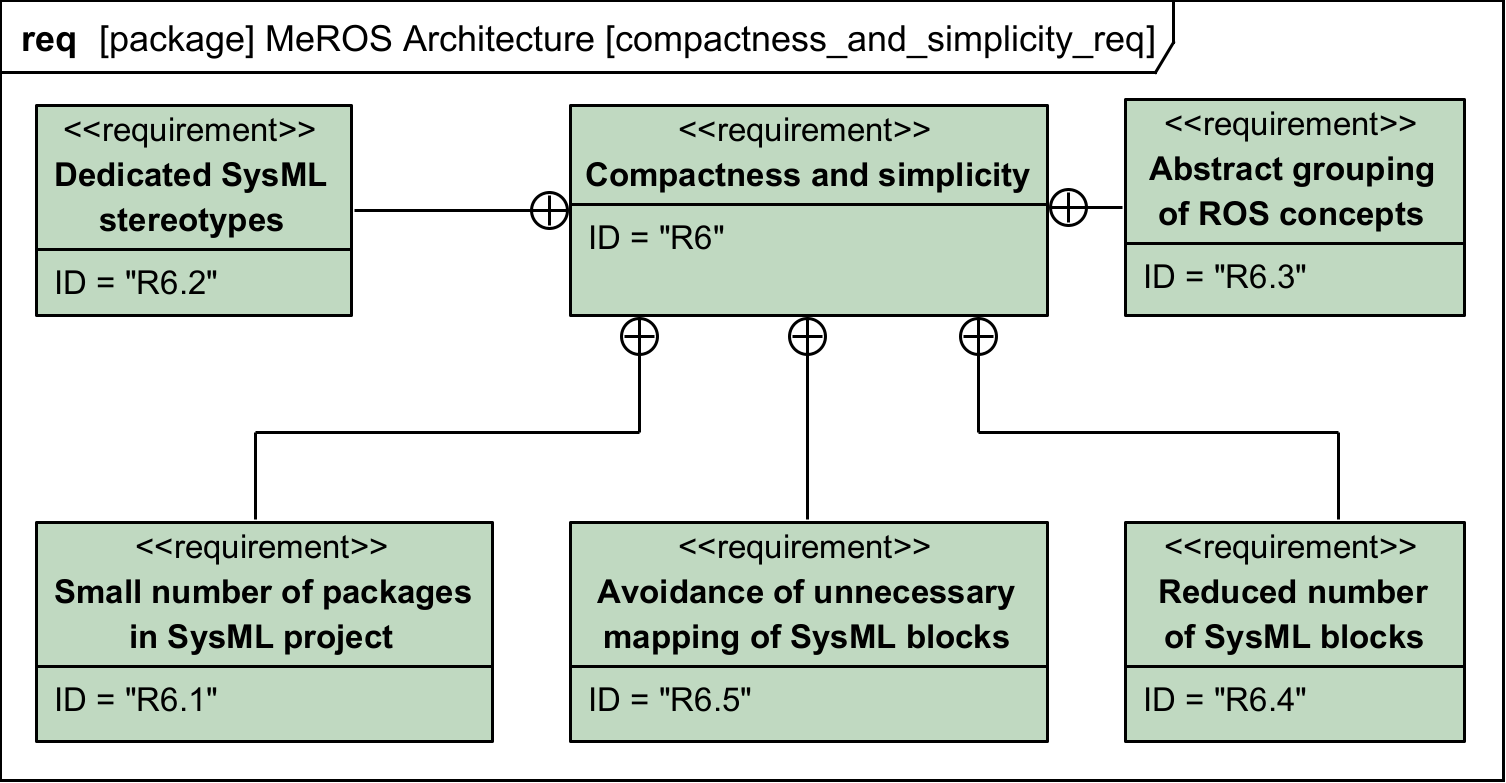
\includegraphics[scale=1.0]{diagrams/compactness_and_simplicity_req.png}}
		\end{center}
		\caption{Compactness and simplicity requirements.  \twci{tutaj 6.3 nie pasuje. Coś trzeba z tym zrobić.}} 
		\label{fig:compactness_and_simplicity_req}
	\end{figure}
	
	A SysML project to develop and represent MeROS metamodel should consist of a~small number of packages [R6.1], but still, the packages should distinguish the major aspects of development process: (i) metamodel requirements formulation, (ii) metamodel itself, and (iii) metamodel realizations/applications.
	Dedicated SysML stereotypes [R6.2] are introduced to MeROS to replace the direct block specialization representation on diagrams and improve the legibility and compactness of diagrams.
	The grouping of concepts [R6.3] has diverse aims. It enables the presentation of the system part in a~general, PIM-like abstract way, on the logical level rather than a~detailed, PSM-like implementation one. The aggregation reduces the number of objects represented on the diagram to highlight the essential aspects and stay compact and consistent in presentation.
	The number of SysML blocks should be reduced to a~reasonable level [R6.4]. Both [R6.1] and [R6.4] help in the Avoidance of unnecessary mapping of SysML blocks [R6.5].

	
	
\chapter{MeROS metamodel}
\label{ch:metamodel}

	\twci{Do aktualizacji. Teraz będą dwie dokumentacje. Oddzielnie dla metamodelu i oddzielnie dla przykłądu z turtlesimem. W tym przykładzie będzie omówienie jak on powstawał, w sensie dodatkowych zrzutów ekranu z retrospekcji działającego systemu ROS. Czyli pokazujemy jak za pomocą rowowych komend uzyskać informacje potrzebne do stworzenia modelu. Jest to bezcenne na ANRO i nie tylko.}
	
	MeROS metamodel is formulated according to the requirements discussed in the previous section. Sec.~\ref{sec:metamodel-composition} presents MeROS blocks' structural composition, and sec.~\ref{sec:metamodel-communication} describes inter-component communication. From the metamodel perspective, the structural aspects [R2] are formulated in both sections, while behavioural [R1] is in the latter. The diagrams comprise selected requirements being allocated to expose the MeROS metamodel development process. 
	
	The MeROS diagrams were created in the Enterprise Architect development tool within the SysML project [R8] and organised in three packages [R6.1] (Fig.~\ref{fig:meros_project_packages_pkg}): (i) Requirement Model related to requirements formulation and analysis, (ii) MeROS -- the metamodel itself, (iii) Rico Controller -- the exemplary ROS~1 application of MeROS described in sec.~\ref{ch:application-example}. 
	
	
	
	The stereotypes are introduced in MeROS metamodel [R6.2].
	The stereotypes names are created to compromise the descriptiveness and short length. Hence, the ROS phrase is avoided in stereotypes as long as there is only the ROS concept of a~given type.
	
	
	
\section{Metamodel composition}
\label{sec:metamodel-composition}

	The degree of specificity of a~metamodel is a~compromise between its comprehensiveness (and, therefore, more general formulation) and a~more accurate representation of a~particular subclass of specific implementations. The metamodel contains compositions of elements and other primary relationships. Attributes and operations range widely, in particular between ROS~1 and ROS~2. Hence, their inclusion would lead to overgrowth and complication of the metamodel [R6]. The MeROS Metamodel is lightweight and general for various system development procedures and non-ROS parts of the whole System. The fundamental decision was to make it compact, so due to the extremely wide range of Non-ROS context variants [R9], they are specific for particular applications and are not specified in the metamodel itself.
	Hence, models derived from the metamodel can define their stereotypes, operations and new relations specific to a~particular System. 
	
	
	The SysML blocks reflect ROS concepts [R3], and their composition is depicted in bdd (block definition diagrams). The metamodel is formulated in a~single SysML package. Hence blocks, i.e., Sources Containers (specialised especially by Workspaces) and Running System Components are composed into System (Fig.~\ref{fig:ros_system_bdd}). The Communication Channel as as specialisation of the System is introduced to specify communication between various Communicating Components. Hardware block reflects to embodiment [R11]. System can aggregate other Systems.
	
		
	\begin{figure}[H]
		\centering
		\begin{center}
			{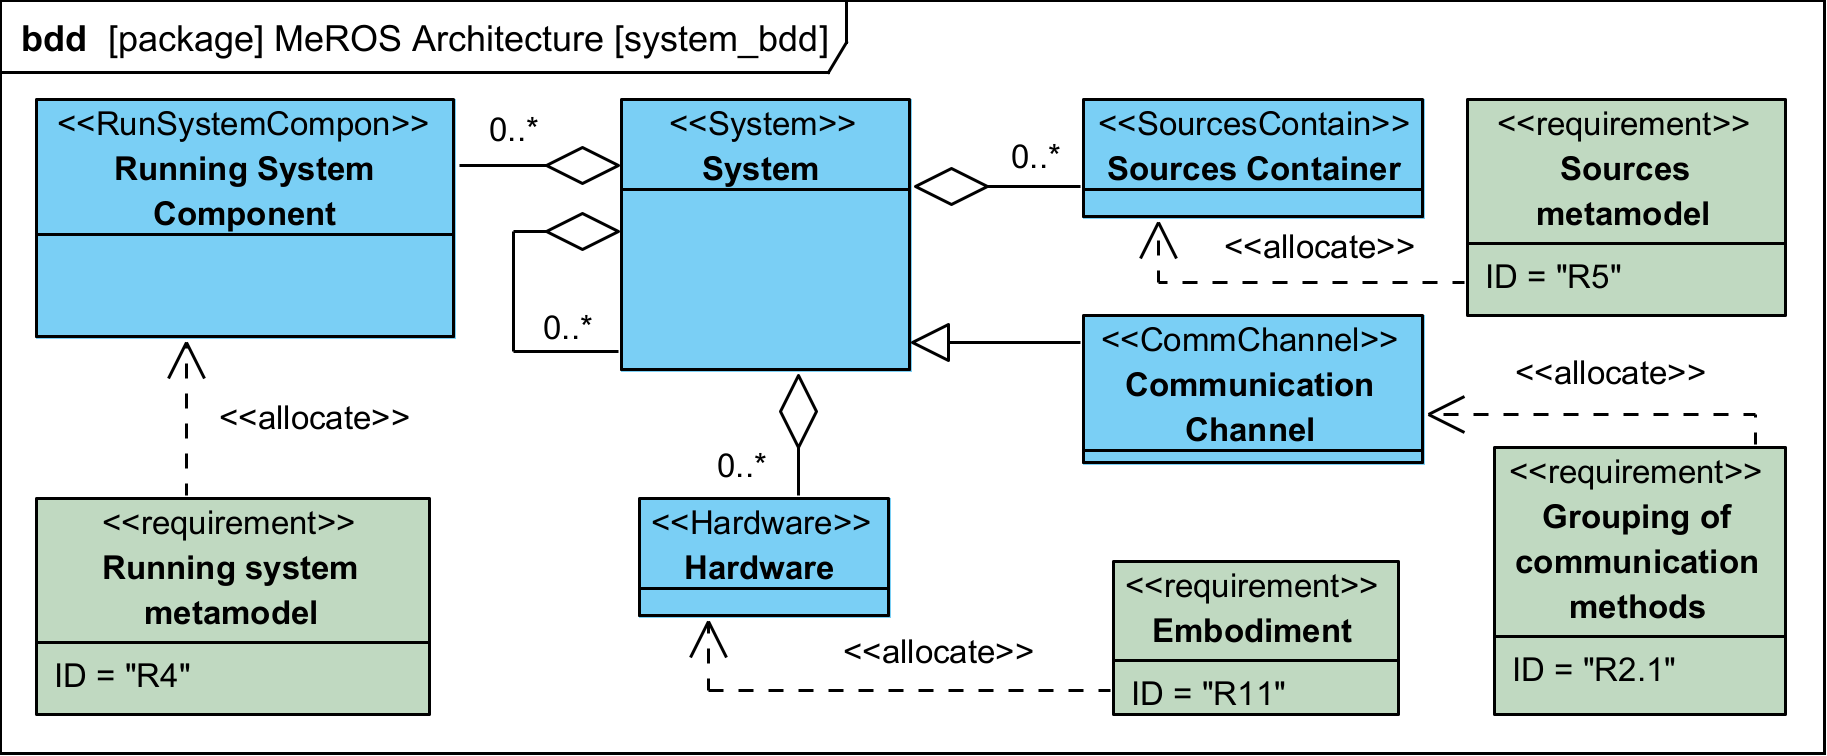
\includegraphics[scale=1.0]{diagrams/system_bdd.png}}
		\end{center}
		\caption{System general composition.  \twci{dlaczego system nie zawiera metod komunikacji?}} 
		\label{fig:ros_system_bdd}
	\end{figure}
	
	Consequently, some concepts (e.g., Node), a~specialisations of Running System Component, occur in Sources Containers. It reduces the number of SysML blocks in the metamodel [R6.4] and eliminates the need for unnecessary mapping of SysML blocks [R6.5].
		
	\pagebreak	
		
	In MeROS, a~gro (Fig.~\ref{fig:communicating_components_bdd}) is a~crucial abstraction of a~number of ROS concepts to represent their standardised role regarding communication. 
	
		
	\begin{figure}[H]
		\centering
		\begin{center}
			{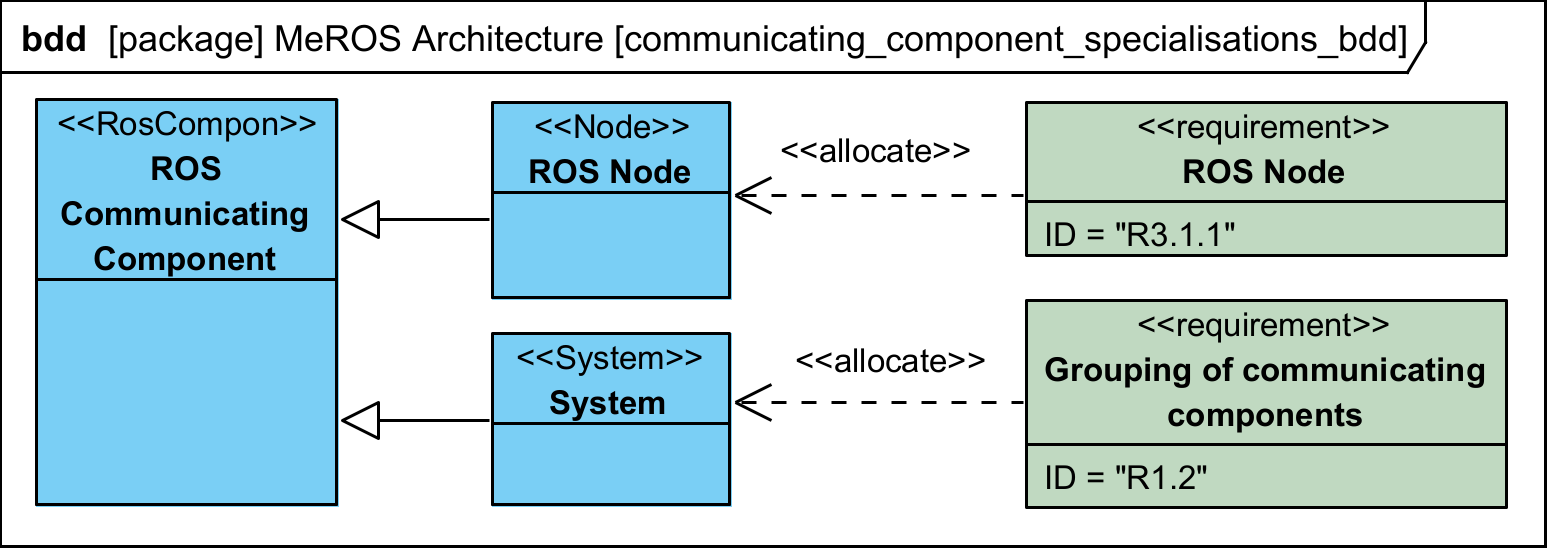
\includegraphics[scale=1.0]{diagrams/communicating_component_specialisations_bdd.png}}
		\end{center}
		\caption{Communicating Component and specialised blocks -- bdd. \twci{może nazwa do skrócenia, żeby diagram nie był sztucznie poszerzony przez długą nazwę diagramu w etykiecie na górze}} 
		\label{fig:communicating_components_bdd}
	\end{figure}
	
	It should be noted that behavioural aspects of a~particular model specified in MeROS can be formulated by operation specification as an act (activity), sd (sequence), or stm (state machine) diagrams. 
	
	
	For clarity, relations of Communicating Components are depicted in several diagrams. Fig.~\ref{fig:communicating_component_topics_bdd} considers Topics and their Data Structures. Here, the ROS Communicating Component can act as a~publisher or a~subscriber.	
	 
	
	\begin{figure}[H]
		\centering
		\begin{center}
			{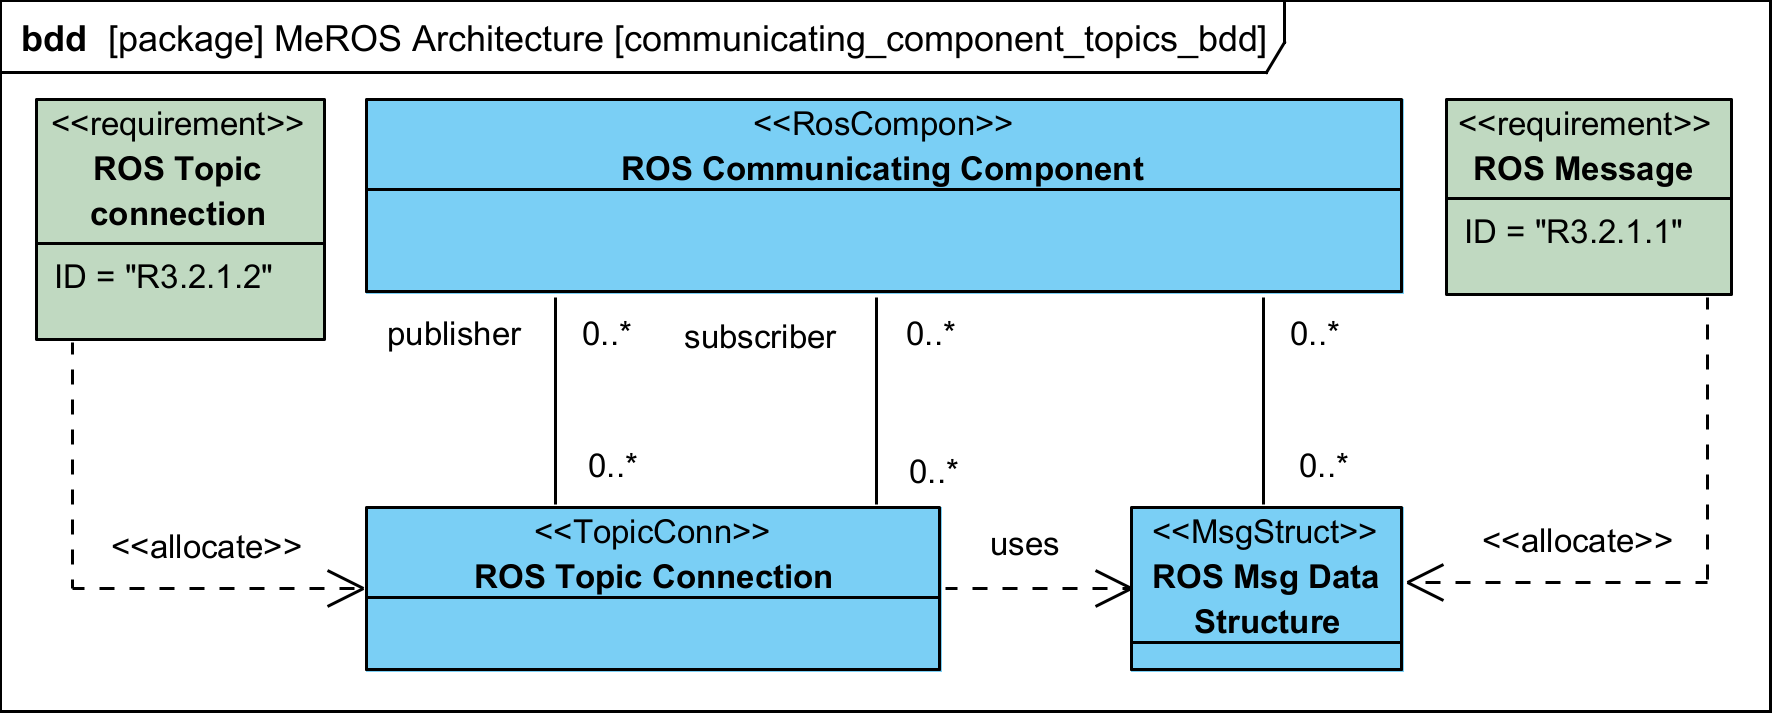
\includegraphics[scale=1.0]{diagrams/communicating_component_topics_bdd.png}}
		\end{center}
		\caption{ROS Communicating Component relations -- Topics.} 
		\label{fig:communicating_component_topics_bdd}
	\end{figure}
	
	\pagebreak
	
	Fig.~\ref{fig:communication_blocks_services_bdd} depicts Services and their Data Structures. In this case, the ROS Communicating Component can act as a~server or a~client.	
	
		
	\begin{figure}[H]
		\centering
		\begin{center}
			{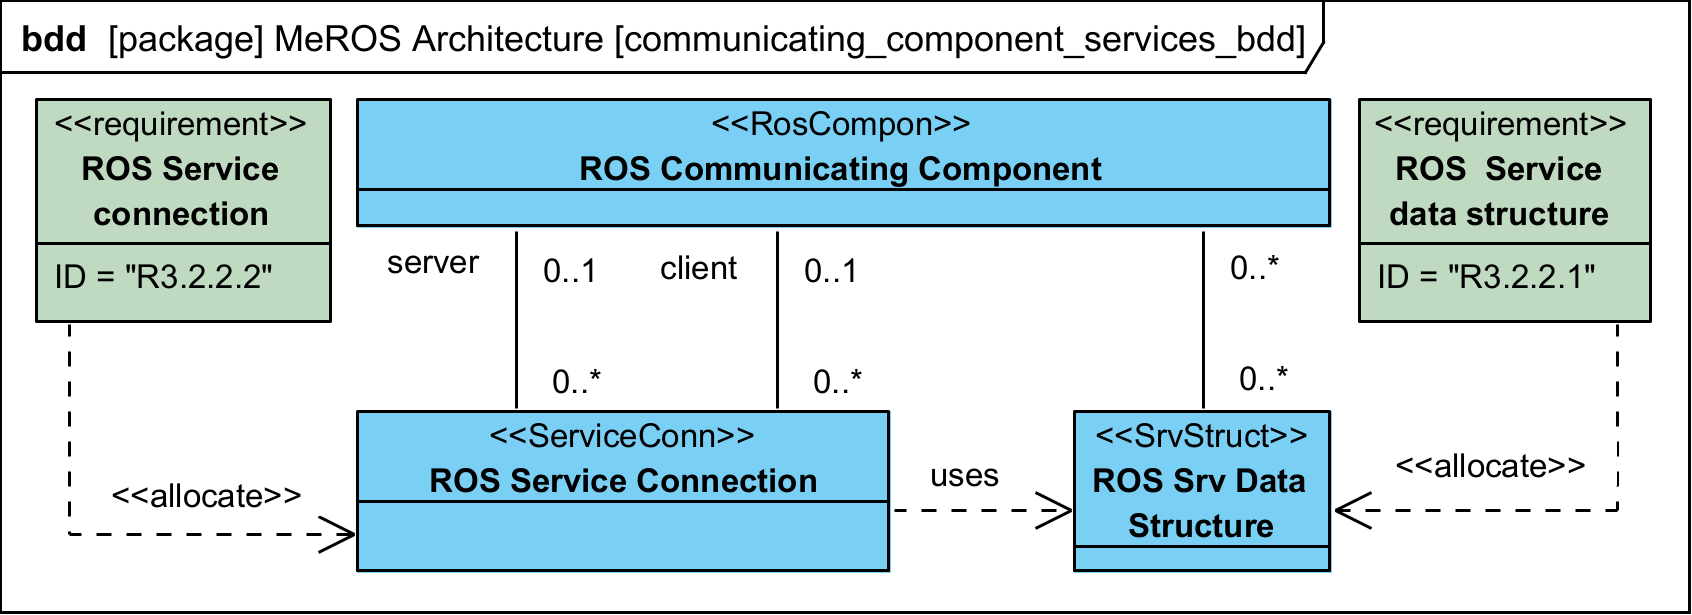
\includegraphics[scale=1.0]{diagrams/communicating_component_services_bdd.png}}
		\end{center}
		\caption{ROS Communicating Component relations -- Services.} 
		\label{fig:communication_blocks_services_bdd}
	\end{figure}
	
	In ROS~2, an Action bases on Topics and Services.
	
	
	The Actions are depicted in two diagrams -- Fig.~\ref{fig:communicating_component_actions_bdd} and Fig.~\ref{fig:action_bdd}. Similarly to Services, the ROS Communicating Component can act as a~server or a~client.	 
	
	
	\begin{figure}[H]
		\centering
		\begin{center}
			{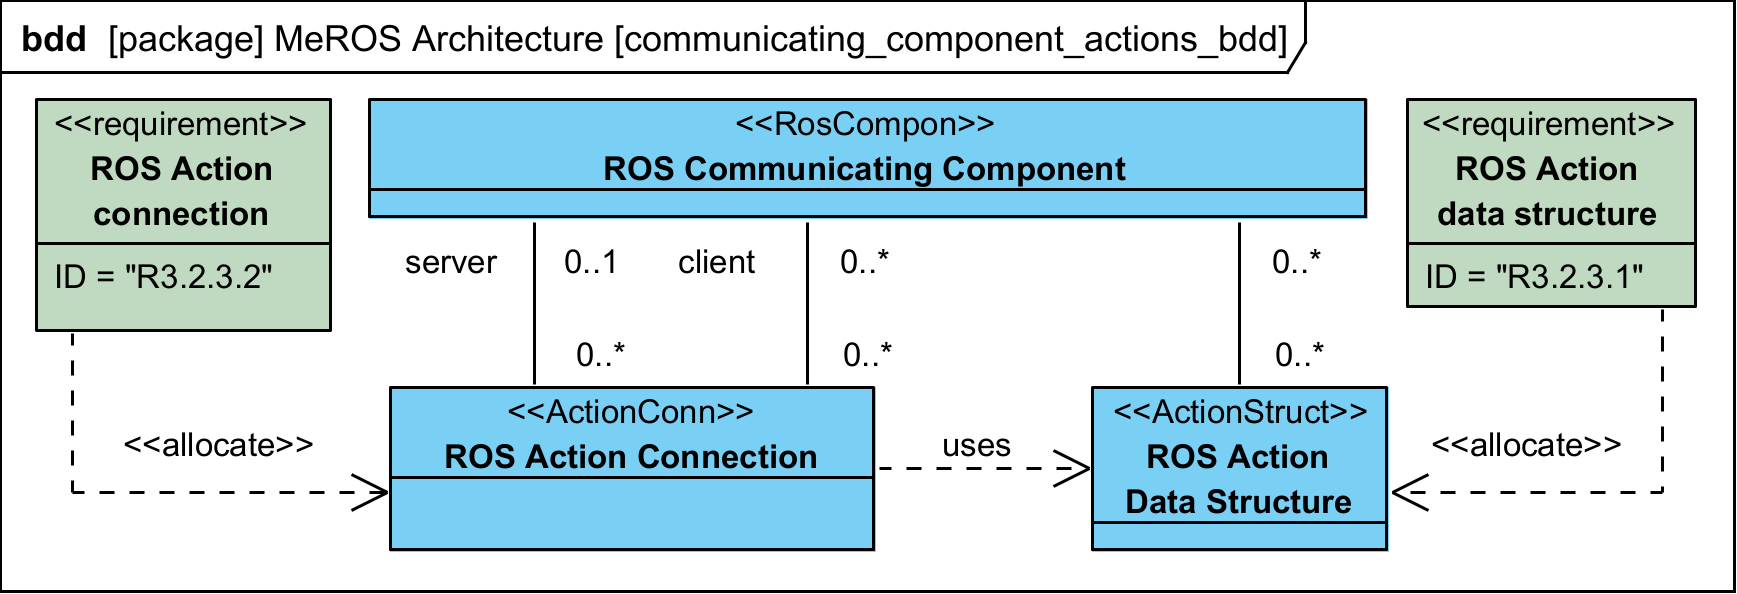
\includegraphics[scale=1.0]{diagrams/communicating_component_actions_bdd.png}}
		\end{center}
		\caption{ROS Communicating Component relations -- Actions.} 
		\label{fig:communicating_component_actions_bdd}
	\end{figure}
	
	An Action Data Structure comprises data used by three of five Topics composed in Action, i.e., goal, feedback and result. Two remaining Topics, i.e., cancel and status are standardised.
	
	\begin{figure}[hbt]
		\centering
		\begin{center}
			{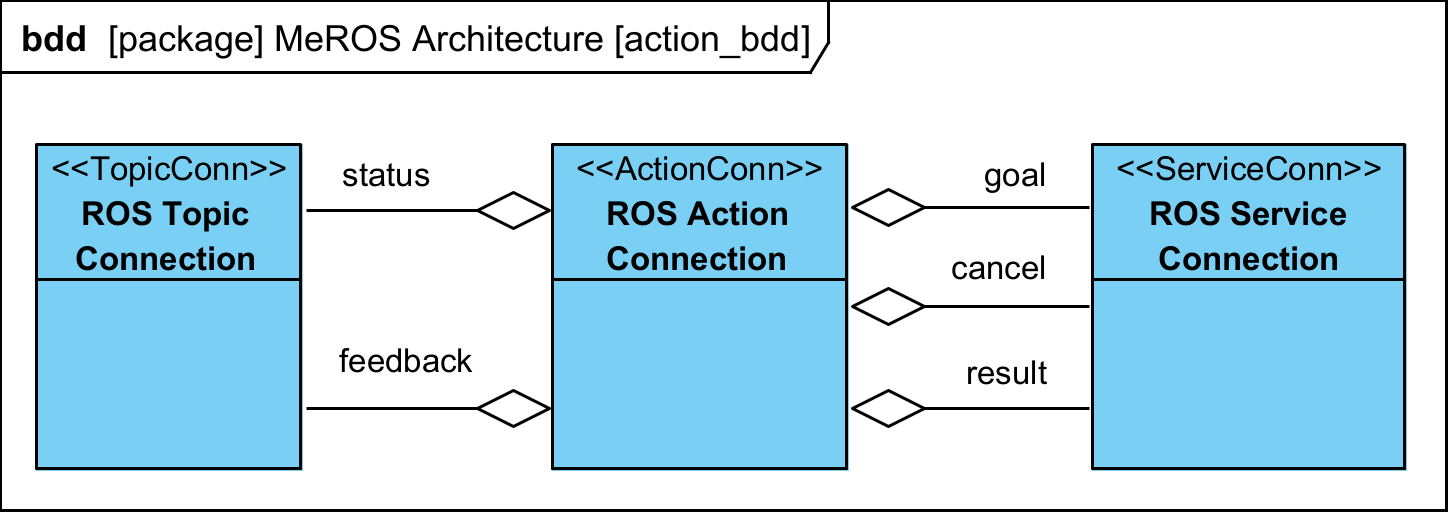
\includegraphics[scale=1.0]{diagrams/action_bdd.png}}
		\end{center}
		\caption{Action.} 
		\label{fig:action_bdd}
	\end{figure}
	
	\pagebreak
	Fig.~\ref{fig:communicating_component_other_bdd} describes how Non-ROS elements are taken into account in relation to communication. Additionally, the figure presents Communication Channel relation to ROS Communicating Component. Besides standard ROS communication methods, the Non-ROS are also included (e.g., http request) to achieve interfaces with Non-ROS parts of the general system. 
	

	\begin{figure}[H]
		\centering
		\begin{center}
			{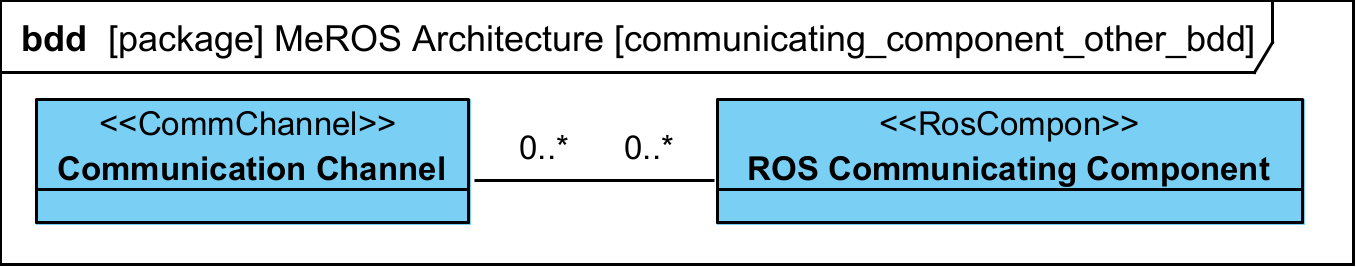
\includegraphics[scale=1.0]{diagrams/communicating_component_other_bdd.png}}
		\end{center}
		\caption{ROS Communicating Component relations -- bdd.} 
		\label{fig:communicating_component_other_bdd}
	\end{figure}
	

	\pagebreak
		 
 	The Node (Fig.~\ref{fig:node_bdd}) composes Parameters and Nodelets (the latter in ROS~1). Two specific Nodes are considered in the metamodel: ROS Master and rosout. In ROS~2, Component Container aggregates Nodes executed in a~single process. The Micro ROS was also considered in the model. 
 	

	 
 	\begin{figure}[H]
	 	\centering
	 	\begin{center}
	 		{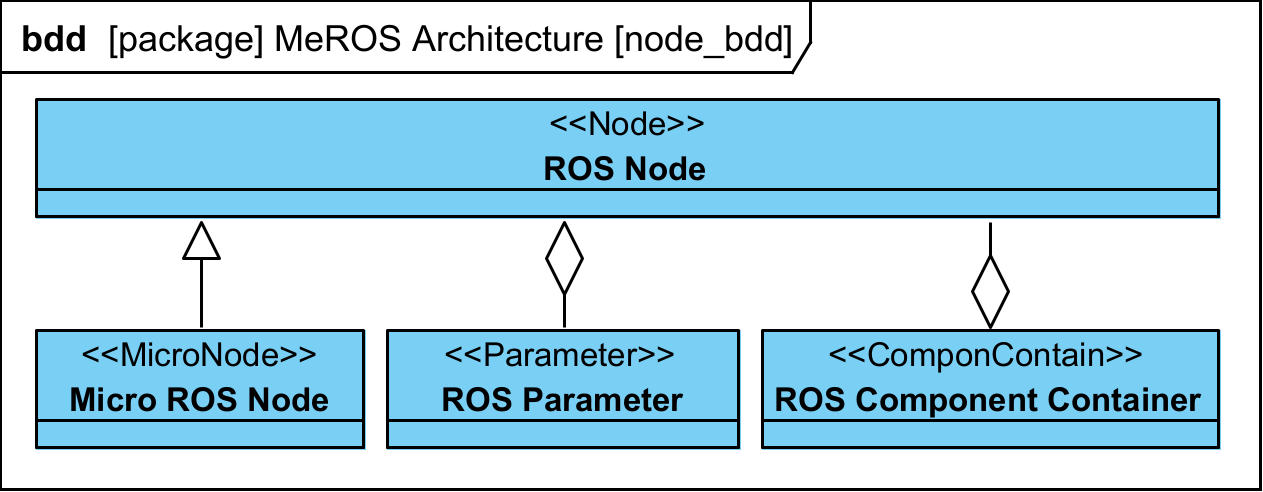
\includegraphics[scale=1.0]{diagrams/node_bdd.png}}
	 	\end{center}
	 	\caption{Node.} 
		 	\label{fig:node_bdd}
	 \end{figure}
	 
	The Running System Component (Fig.~\ref{fig:running_system_component_bdd}) is a~generalisation of Communicating Components specializations as well as Connections between them.
	

	\begin{figure}[H]
		\centering
		\begin{center}
			{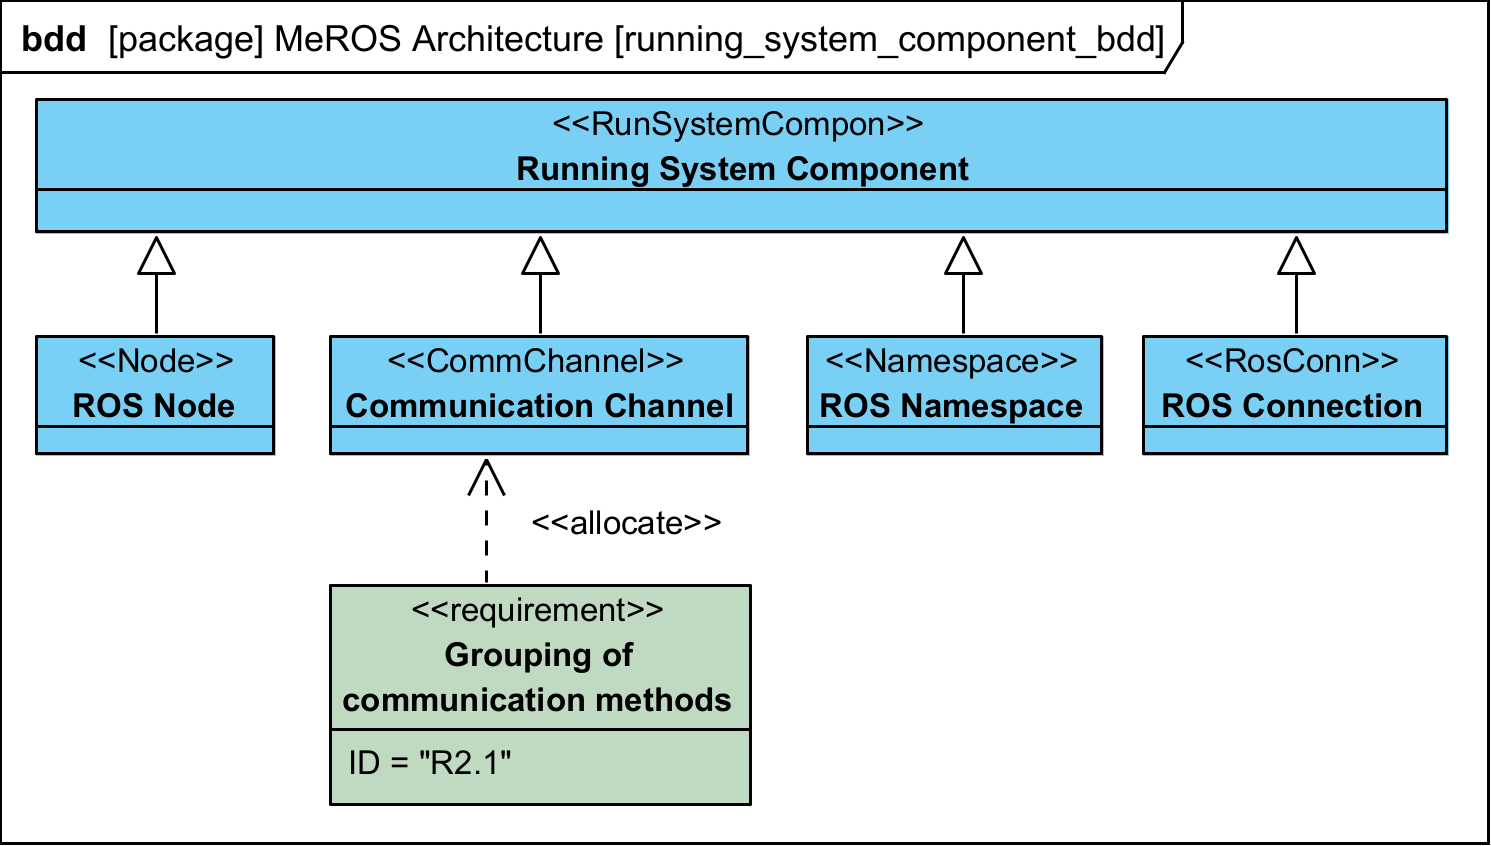
\includegraphics[scale=1.0]{diagrams/running_system_component_bdd.png}}
		\end{center}
		\caption{Running System Component specialisations. \twci{Dziwne jakieś. }} 
		\label{fig:running_system_component_bdd}
	\end{figure} 
	 	 

	It should be noted that although MeROS could be classified as PSM, the initial, general system description with Communications Channels and general Running System corresponds to PIM specification. Then, the detailing of these aggregates corresponds to the transition from PIM to PSM. 
	
		
%	The way Communicating Components use various types of connections is presented in Fig.~\ref{fig:system_communication_bdd}. Both ROS and Non-ROS Communicating Components can communicate via Non-ROS Connections, but only ROS Communicating Components use ROS Connections.
%
%
%	\begin{figure}[H]
%		\centering
%		\begin{center}
%			{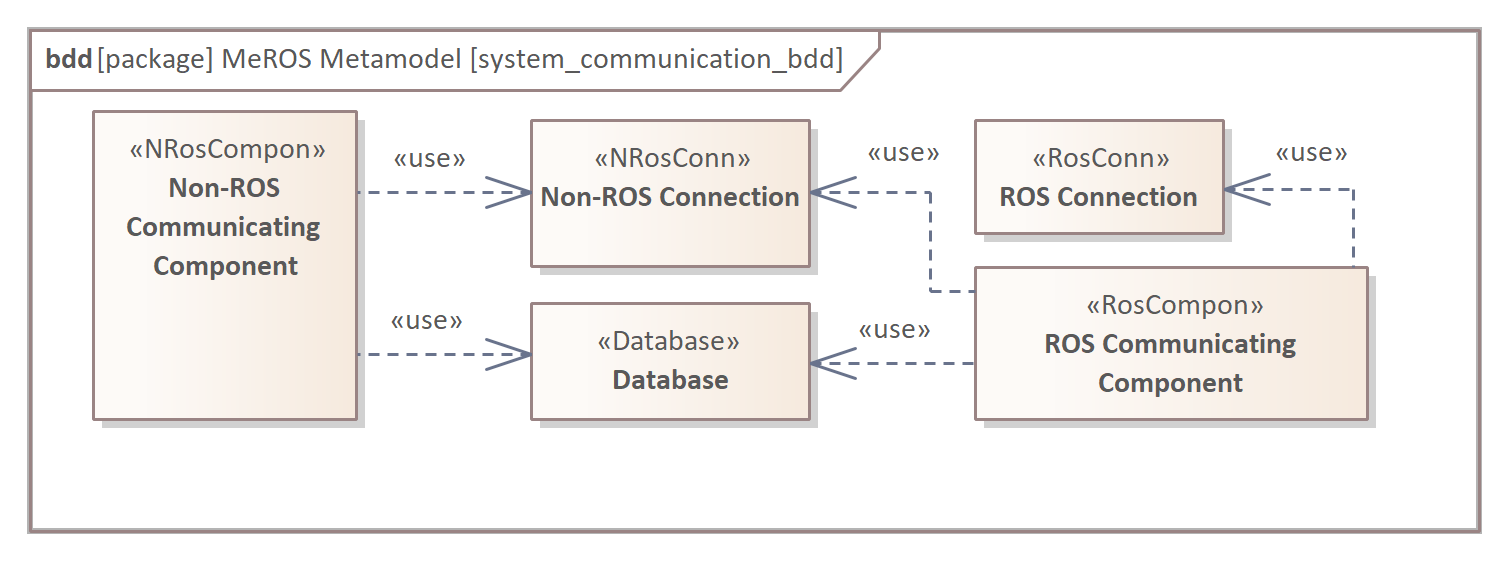
\includegraphics[scale=1.15]{img/meros_pkg/system_communication_bdd.png}}
%		\end{center}
%		\caption{System communication.} 
%		\label{fig:system_communication_bdd}
%	\end{figure}
	
		 The specializations of ROS connection (Topic connections, Service connections, and Action connections) are depicted in Fig.~\ref{fig:ros_connections_bdd}. 
	
	
	\begin{figure}[H]
		\centering
		\begin{center}
			{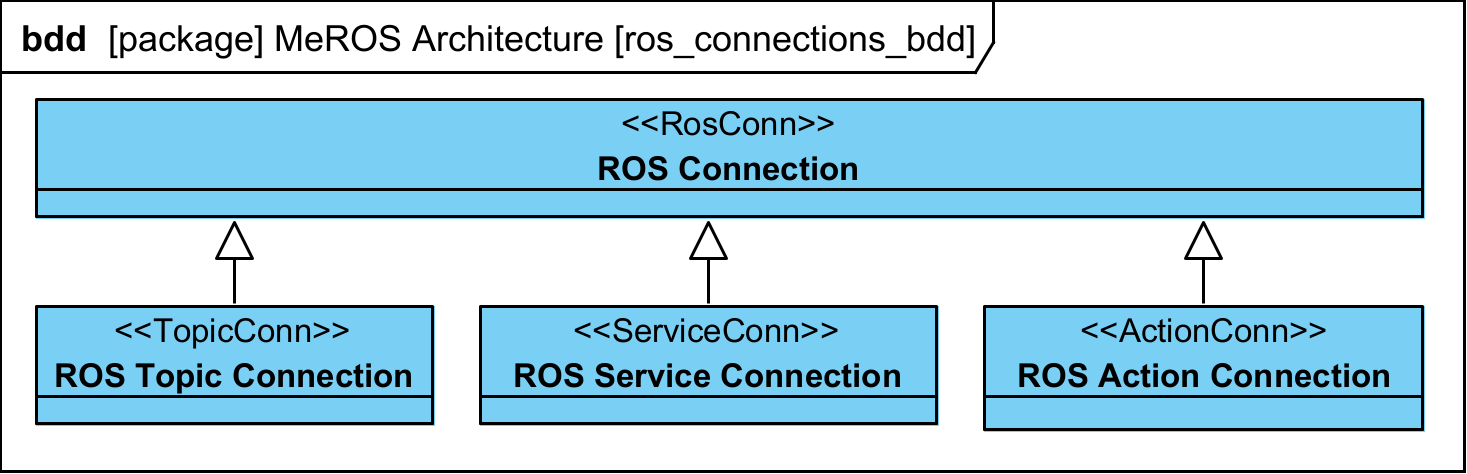
\includegraphics[scale=1.0]{diagrams/ros_connections_bdd.png}}
		\end{center}
		\caption{ROS Connections.} 
		\label{fig:ros_connections_bdd}
	\end{figure}

	
	The Namespace (Fig.~\ref{fig:namespace_bdd}) aggregates elements of the System, but only ROS related. In opposition to the System, the Namespace does not specialise Communicating Component. Hence, it can not act as Communicating Component.
	
	
	\begin{figure}[H]
		\centering
		\begin{center}
			{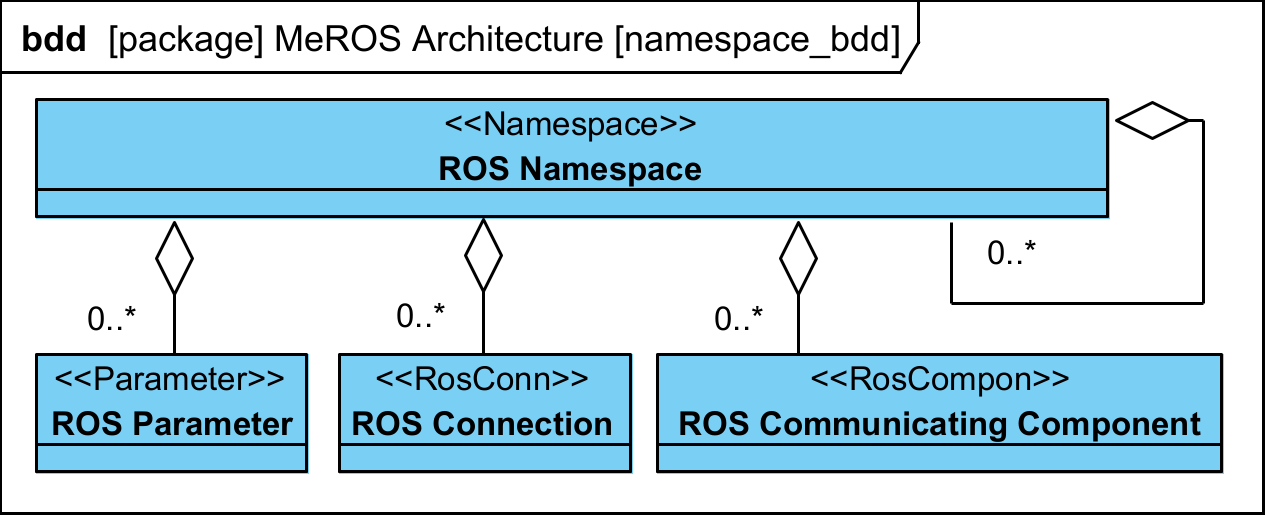
\includegraphics[scale=1.0]{diagrams/namespace_bdd.png}}
		\end{center}
		\caption{Namespace composition.}
		\label{fig:namespace_bdd}
	\end{figure}
	
	The Sources Container (Fig.~\ref{fig:sources_container_bdd}) has various specialisations such as Group of Packages, ROS Workspace, ROS Package and Repository. It also plays a~role of general container.  
	The Workspace contains, i.a., Packages that compose the files related to general ROS concepts such as Node source codes, communication structures definitions, etc. As Workspace has a~specific file-system nature with various types of files stored, Group of Packages were introduced as specific aggregation of ROS Packages only.
	
	
	\begin{figure}[H]
		\centering
		\begin{center}
			{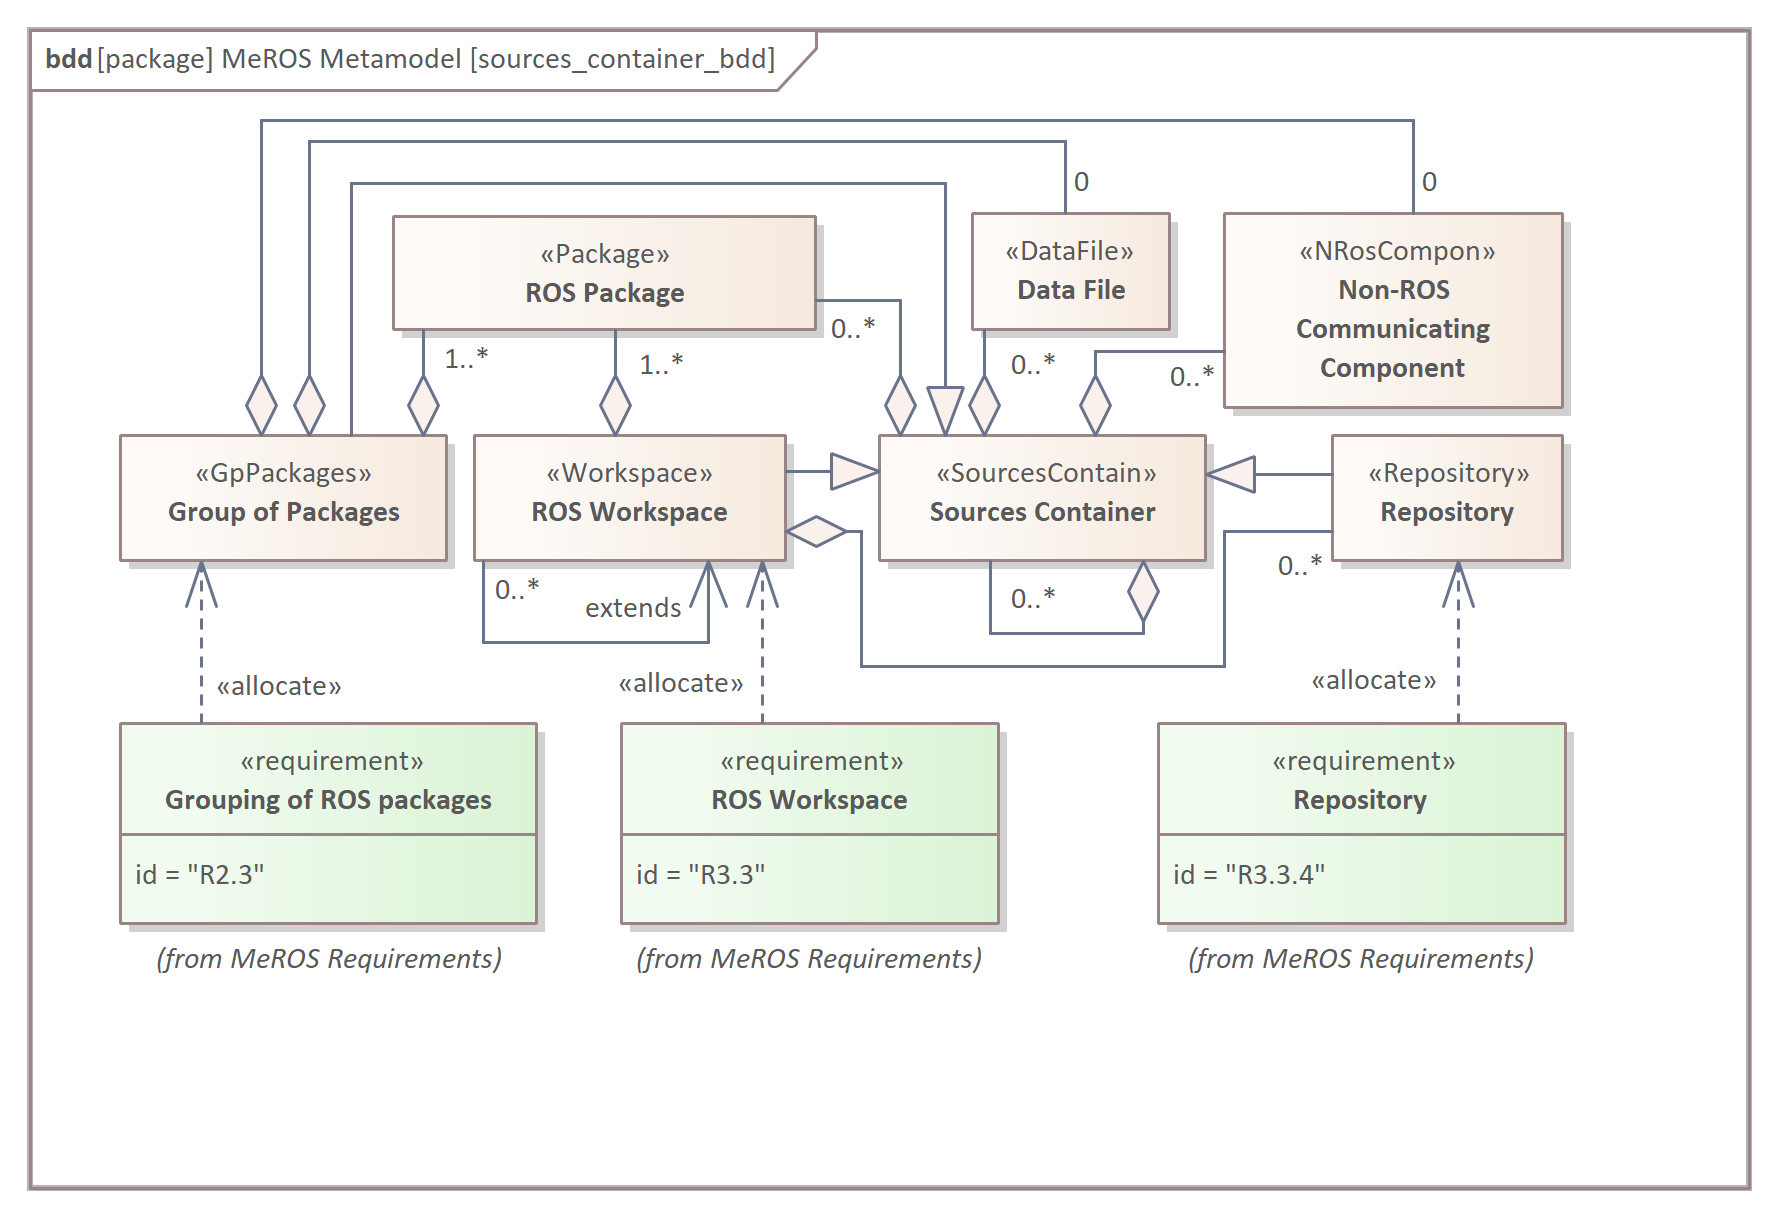
\includegraphics[scale=1.0]{img/meros_pkg/sources_container_bdd.png}}
		\end{center}
		\caption{Sources Container and its specialisations.} 
		\label{fig:sources_container_bdd}
	\end{figure}
	
	The ROS Package (Fig.~\ref{fig:ros_package_bdd}) composes the files related to general ROS concepts such as Node source codes, communication structures definitions, etc. It should be noted that in case of Actions, specific communication structures definitions are stored in Action Data Structures. ROS Meta Package was introduced as a~specific ROS Package specialisation.
	
	\begin{figure}[H]
		\centering
		\begin{center}
			{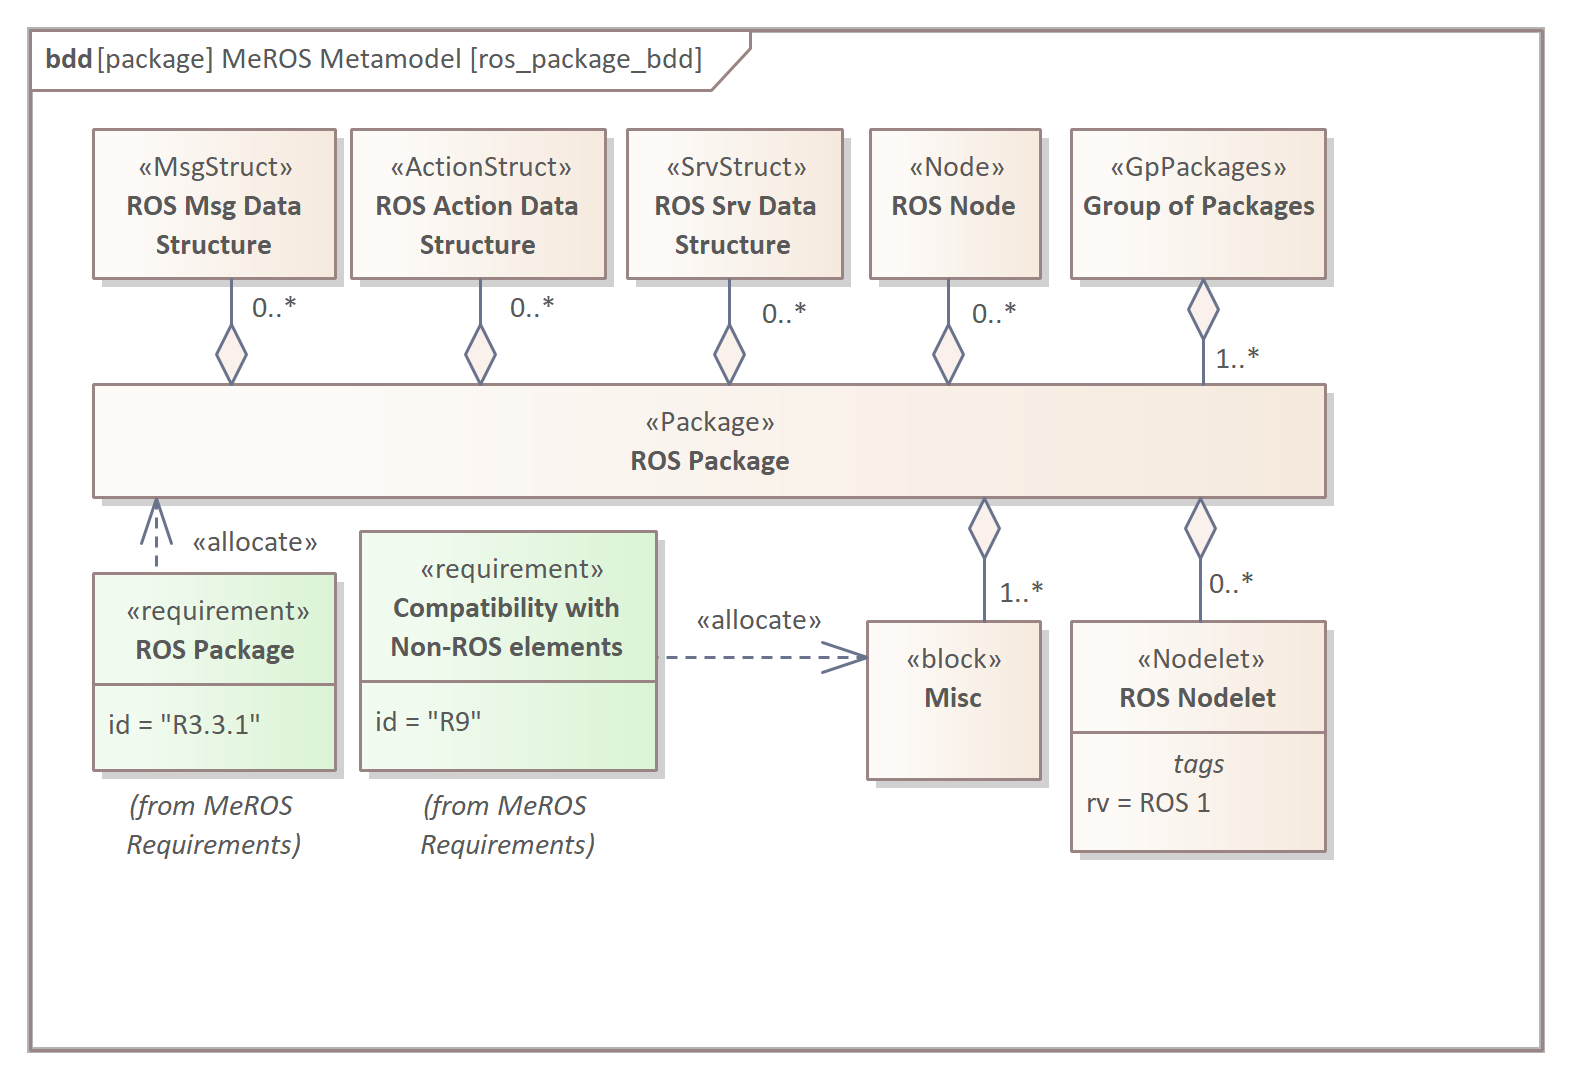
\includegraphics[scale=1.0]{img/meros_pkg/ros_package_bdd.png}}
		\end{center}
		\caption{ROS Package composition.} 
		\label{fig:ros_package_bdd}
	\end{figure}
		
		
%The composition of Versatile Sources Container is presented in Fig.~\ref{fig:ver_sources_contain_bdd}.
%
%	\begin{figure}[H]
%		\centering
%		\begin{center}
%			{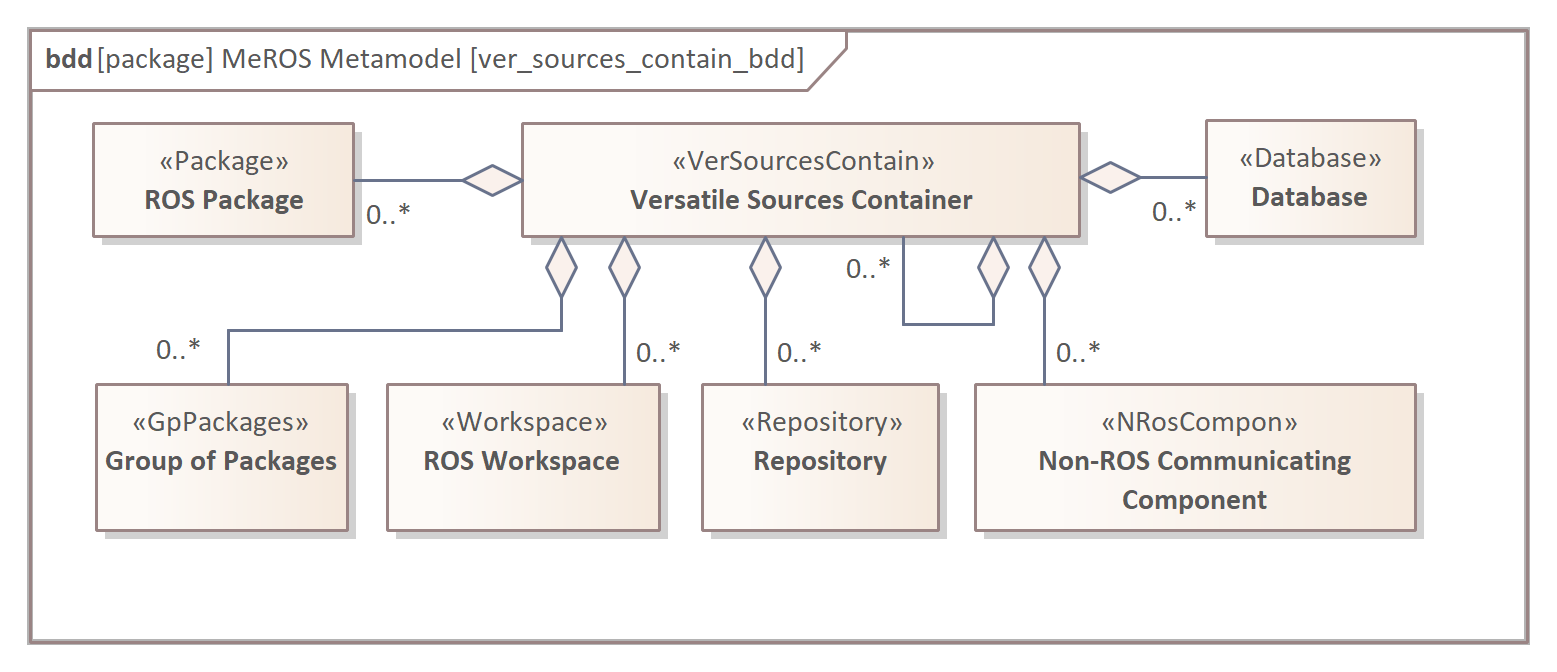
\includegraphics[scale=1.0]{img/meros_pkg/ver_sources_contain_bdd.png}}
%		\end{center}
%		\caption{Versatile Sources Container composition.} 
%		\label{fig:ver_sources_contain_bdd}
%	\end{figure}
	
The composition of Repository is presented in Fig.~\ref{fig:repository_bdd}.	
	
	\begin{figure}[H]
		\centering
		\begin{center}
			{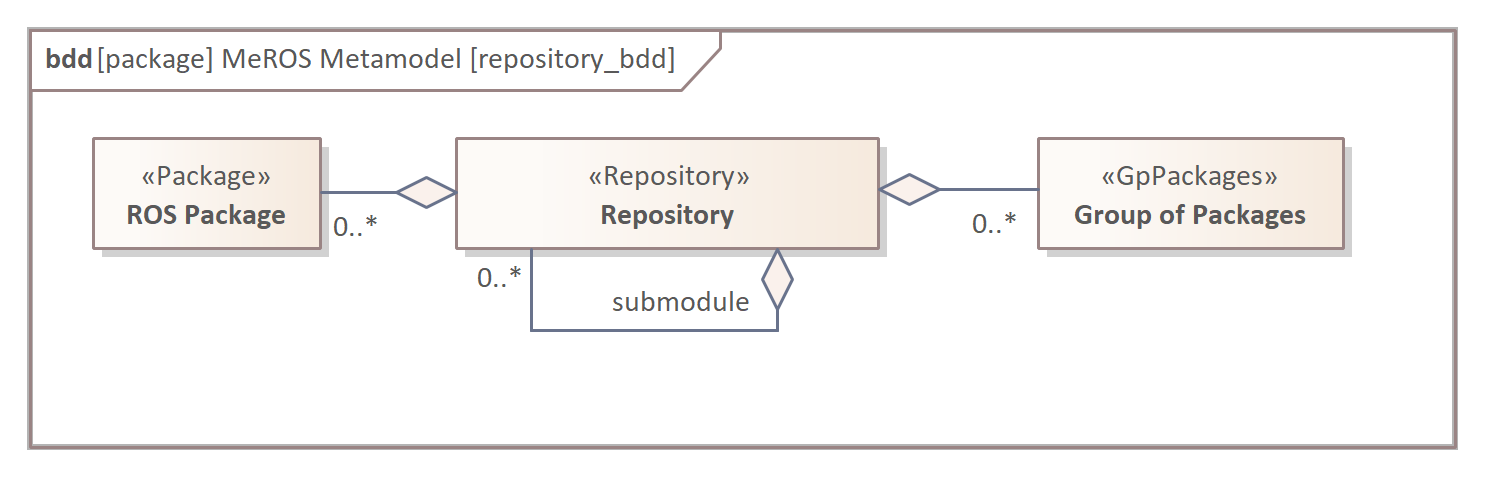
\includegraphics[scale=1.0]{img/meros_pkg/repository_bdd.png}}
		\end{center}
		\caption{Repository composition.} 
		\label{fig:repository_bdd}
	\end{figure}

The composition of ROS Workspace is presented in Fig.~\ref{fig:ros_workspace_bdd}.

	\begin{figure}[H]
		\centering
		\begin{center}
			{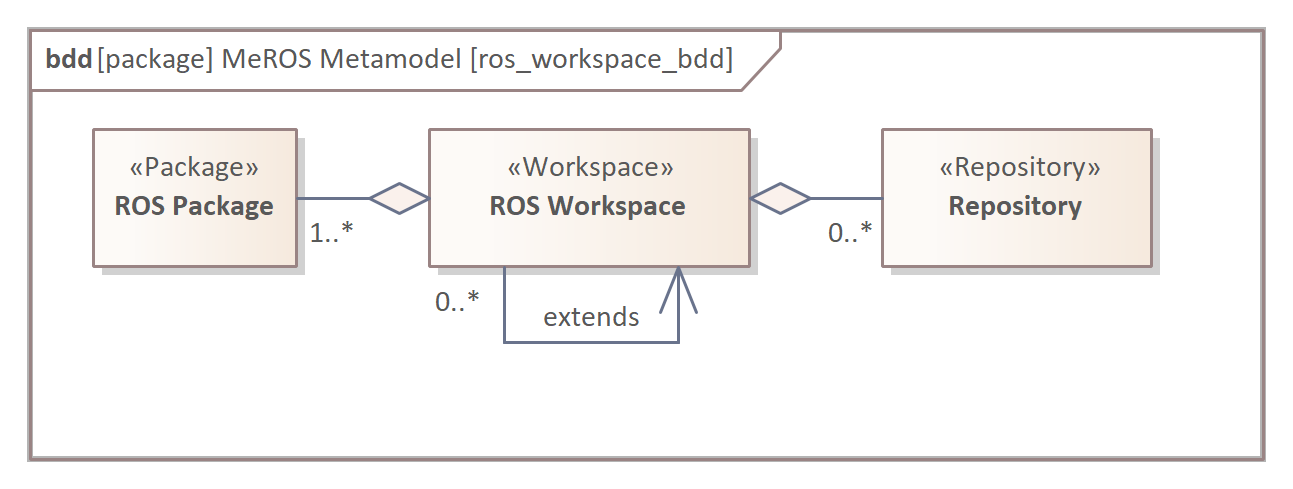
\includegraphics[scale=1.0]{img/meros_pkg/ros_workspace_bdd.png}}
		\end{center}
		\caption{ROS Workspace composition.  \twci{dlaczeggo worskapce nie agraguej grupy pakietów?}} 
		\label{fig:ros_workspace_bdd}
	\end{figure}
	
\pagebreak

\section{Communication}
\label{sec:metamodel-communication}
	
	This section depicts the behavioural and structural aspects of communication in the system. The previous section considers block definition diagrams (bdd). In the following part, the internal block diagrams (ibd) and behavioural diagrams are discussed. The goal is to present three modes of communication: ROS Topic [R4.1] (sec.~\ref{ch:metamodel-topic}), ROS Service [R4.2] (sec.~\ref{ch:metamodel-service}) and ROS Action [R4.3] (sec.~\ref{ch:metamodel-action}). It should be noted that the concept of presentation of communication with and without a~dedicated communication component is illustrated on communication with Topics but can also be applied to Services, Actions and Communication Channels. The dedicated component is especially needed when the particular Communication Channel is at first represented in a~general way as the separated block corresponding to this component, then specified in detail in the internal block diagram. 
	
	\subsection{ROS Topic}
	\label{ch:metamodel-topic}
		
	Fig.~\ref{fig:topic_communication_with_dedicated_component_ibd} presents the ibd diagram of publishers' and subscribers' communication via topics. This diagram uses a~dedicated communication component for each Topic [R4.1.1]. There are no general limits to the number of publishers, subscribers and Topics they communicate with. 
	

	\begin{figure}[H]
		\centering
		\begin{center}
			{\includegraphics[scale=1.1]{img/meros_pkg/topic_communication_with_compon_ibd.png}}
		\end{center}
		\caption{Topics with dedicated communication components -- all components.} 
		\label{fig:topic_communication_with_dedicated_component_ibd}
	\end{figure}

	Thanks to a~dedicated component to represent communication, the diagram in Fig.~\ref{fig:topic_communication_with_dedicated_component_ibd} can be split into two considering publisher (Fig.~\ref{fig:topic_split_publisher_ibd}) and subscriber (Fig.~\ref{fig:topic_split_subscriber_ibd}) separately, without losing information. It is especially useful when system fragments are presented after its decomposition that subdivides communication channels.
	
	
	 \begin{figure}[H]
		\begin{subfigure}[b]{0.49\textwidth}
			\includegraphics[width=\textwidth]{img/meros_pkg/topic_split_publisher_ibd.png}
			\caption{publisher}
			\label{fig:topic_split_publisher_ibd}
		\end{subfigure}
		\begin{subfigure}[b]{0.51\textwidth}
			\includegraphics[width=\textwidth]{img/meros_pkg/topic_split_subscriber_ibd.png}
			\caption{subscriber}
			\label{fig:topic_split_subscriber_ibd}
		\end{subfigure}
		\caption{Topics with dedicated communication components.}
	\end{figure}
	

	
	
%
%	\begin{figure}[H]
%		\centering
%		\begin{center}
%			{\includegraphics[scale=1.0]{img/meros_pkg/topic_split_publisher_ibd.png}}
%		\end{center}
%		\caption{Topics with dedicated communication components -- publisher -- ibd.} 
%		\label{fig:topic_split_publisher_ibd}
%	\end{figure}
%
%
%	\begin{figure}[H]
%		\centering
%		\begin{center}
%			{\includegraphics[scale=1.0]{img/meros_pkg/topic_split_subscriber_ibd.png}}
%		\end{center}
%		\caption{Topics with dedicated communication components -- subscriber -- ibd.} 
%		\label{fig:topic_split_subscriber_ibd}
%	\end{figure}
	
	\pagebreak
	
	Fig. \ref{fig:topic_communication_with_dedicated_component_sd} depicts the corresponding sequence diagram. Publishers send a~message through Topics to the subscribers. The incoming message cause the subscriber to execute the callback function. 
	
	\begin{figure}[H]
		\centering
		\begin{center}
			{\includegraphics[scale=1.0]{img/meros_pkg/topic_communication_with_compon_sd.png}}
		\end{center}
		\caption{Topics with dedicated communication components.} 
		\label{fig:topic_communication_with_dedicated_component_sd}
	\end{figure}
		
	
	Fig.~\ref{fig:topic_communication_without_dedicated_component_ibd} and Fig.~\ref{fig:topic_communication_without_dedicated_component_sd} present an alternative approach to depict the system communicating via topics. In this case, no dedicated communication components are used [R4.1.2]. 
	
	
	\begin{figure}[H]
		\centering
		\begin{center}
			{\includegraphics[scale=1.0]{img/meros_pkg/topic_communication_non_compon_ibd.png}}
		\end{center}
		\caption{Topics without dedicated communication components.} 
		\label{fig:topic_communication_without_dedicated_component_ibd}
	\end{figure}
	
	\begin{figure}[H]
		\centering
		\begin{center}
			{\includegraphics[scale=1.0]{img/meros_pkg/topic_communication_non_compon_sd.png}}
		\end{center}
		\caption{Topics without dedicated communication components.} 
		\label{fig:topic_communication_without_dedicated_component_sd}
	\end{figure}
	
	
	\pagebreak
	
	
\subsection{ROS Service}
\label{ch:metamodel-service}
	
	For each ROS Service, there is at most one server and a~number of clients (Fig.~\ref{fig:service_communication_ibd} and Fig.~\ref{fig:service_communication_sd}). Service-type communication is bidirectional and realises RPC (remote procedure call).
	

	\begin{figure}[H]
		\centering
		\begin{center}
			{\includegraphics[scale=1.1]{img/meros_pkg/service_communication_ibd.png}}
		\end{center}
		\caption{Service-based communication.} 
		\label{fig:service_communication_ibd}
	\end{figure}
	

	\begin{figure}[H]
		\centering
		\begin{center}
			{\includegraphics[scale=1.1]{img/meros_pkg/service_communication_sd.png}}
		\end{center}
		\caption{Service-based communication.} 
		\label{fig:service_communication_sd}
	\end{figure}
	
	
\subsection{ROS Action}
\label{ch:metamodel-action}
	
	ROS Action communication's general, simplified structure (Fig.~\ref{fig:action_communication_compact_ibd}) is analogous to ROS Service. These type of presentation is universal for ROS~1 and ROS~2.
	

	\begin{figure}[H]
		\centering
		\begin{center}
			{\includegraphics[scale=1.1]{img/meros_pkg/action_communication_compact_ibd.png}}
		\end{center}
		\caption{Action-based communication -- compact representation.} 
		% https://docs.ros.org/en/foxy/Tutorials/Beginner-CLI-Tools/Understanding-ROS2-Actions/Understanding-ROS2-Actions.html
		\label{fig:action_communication_compact_ibd}
	\end{figure}
	
	
	 An Action (Fig.~\ref{fig:action_communication_detailed_ibd}) is based on several Topics in ROS~1, while on Topics and Services in ROS~2.
	

	\begin{figure}[H]
		\centering
		\begin{center}
			{\includegraphics[scale=1.0]{img/meros_pkg/action_communication_detailed_ibd.png}}
		\end{center}
		\caption{Action-based communication -- detailed.} 
		% https://design.ros2.org/articles/actions.html
		\label{fig:action_communication_detailed_ibd}
	\end{figure}
	
	In practice, to present an action-related communication compactly on sd diagram (Fig.~\ref{fig:action_communication_compact_sd}) particular Topics and Services can be generalised as a~request (for /goal and /cancel) and a~response (for /status, /feedback and /result). It should be noted that this diagram presents the Action communication sequence in a~simplified way.
	
	\begin{figure}[H]
		\centering
		\begin{center}
			{\includegraphics[scale=1.1]{img/meros_pkg/action_communication_compact_sd.png}}
		\end{center}
		\caption{Action-based communication sequence -- compact presentation.} 
		\label{fig:action_communication_compact_sd}
	\end{figure}

	
	
\chapter{MeROS application}
\label{ch:application}
	
	
	MeROS metamodel can be employed in various ways in broad context of SE. To help to develop projects, the MeROS UML profile and other materials are accessible from MeROS project page\footnote{\url{http://github.com/twiniars/meros}}. 
	
	
\section{Exemplary system}
\label{ch:application-example}

	This section presents key aspects of an exemplary system development process incorporating MeROS. The exemplary system was created within the AAL INCARE project to control the Rico assistive robot (modified TIAGo platform with controller based on ROS~1) to execute transportation attendance tasks (Fig.~\ref{fig:herbatka_u_winiara}).
	
	\begin{figure}[H]
		\centering
		\begin{center}
			{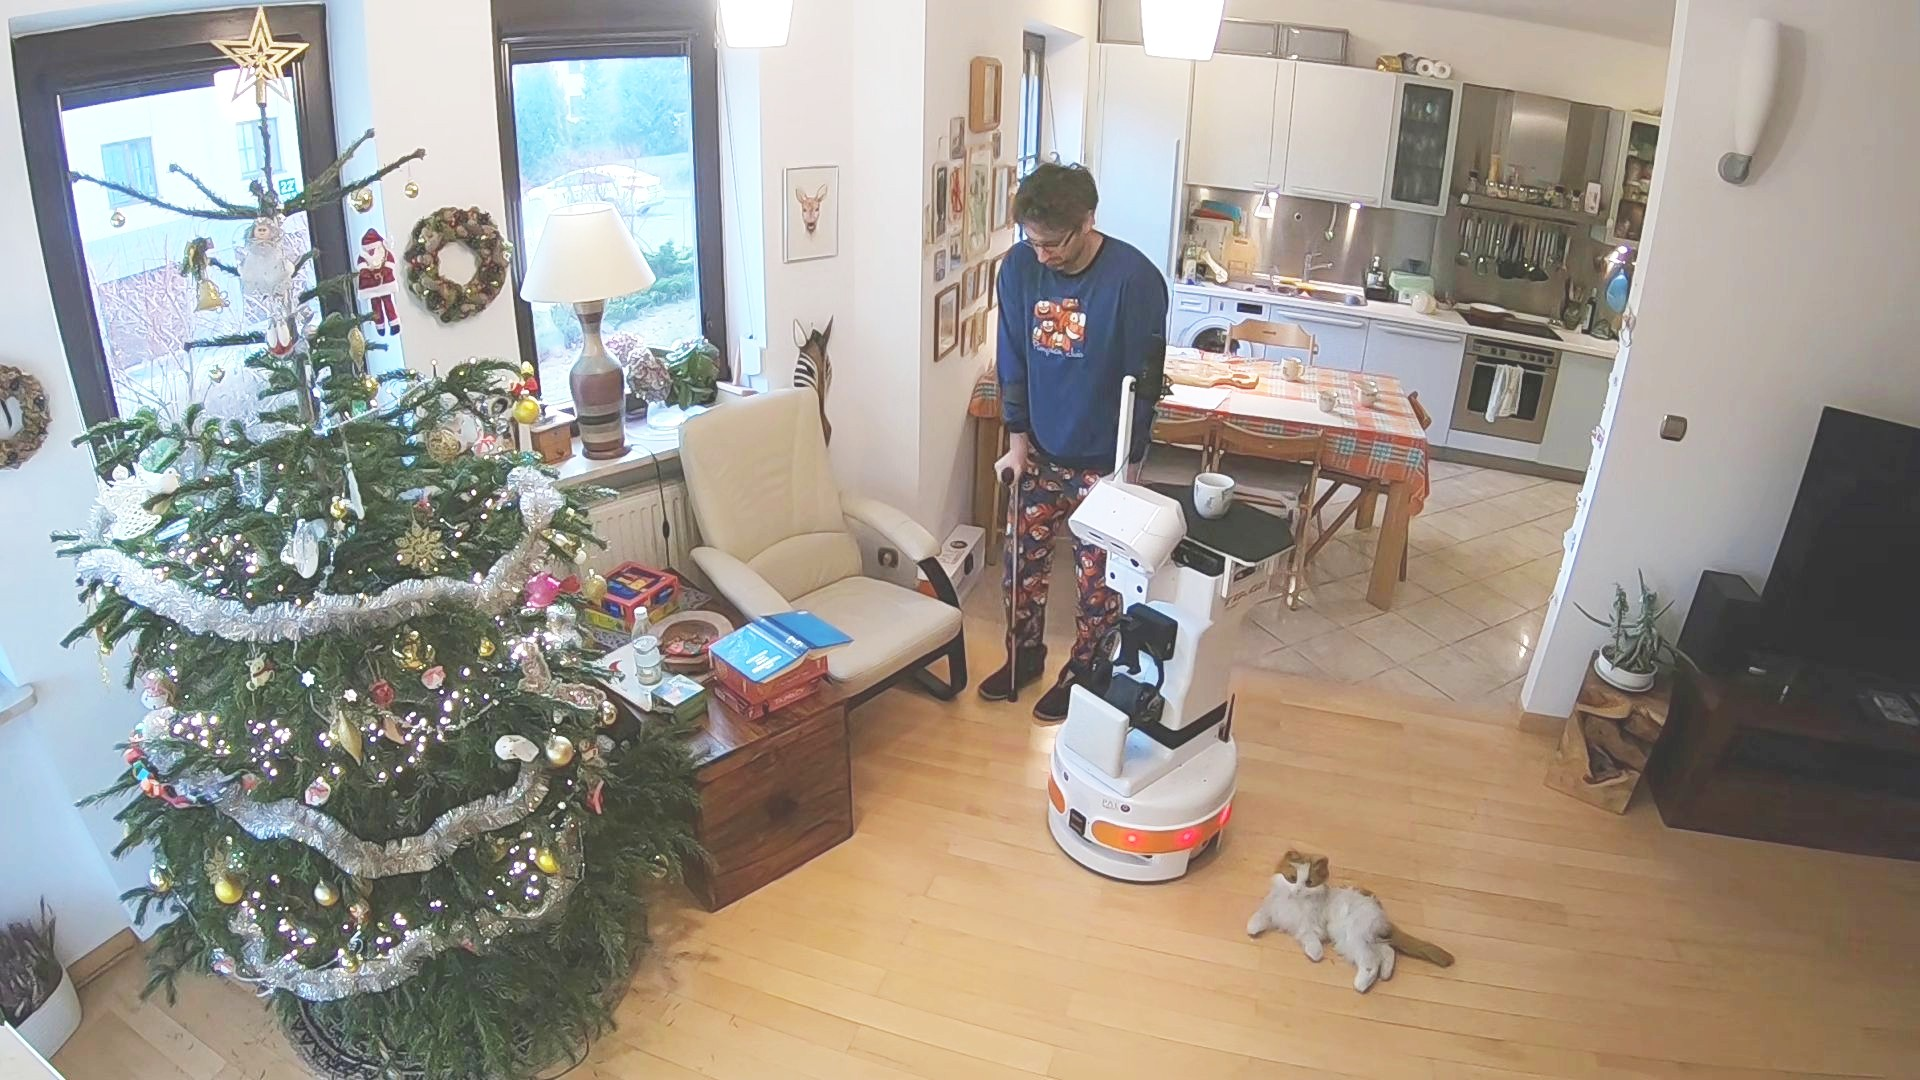
\includegraphics[width=\columnwidth]{img/herbatka_u_winiara.jpg}}
		\end{center}
		\caption{Transportation attendance by Rico robot \url{https://vimeo.com/670252925}} 
		\label{fig:herbatka_u_winiara}
	\end{figure}
	
	
	
	 The purpose of the following description is not to document the entire system but to illustrate, by example, representative aspects of the MeROS application.
	 
	\newpage
	The Rico \stSystem{} consists of two parts. Its \stWorkspace{} and a~number of \stRunSystemCompon{} (Fig.~\ref{fig:rico_system_bdd}).
	
	
	\begin{figure}[H] 
		\centering
		\begin{center}
			{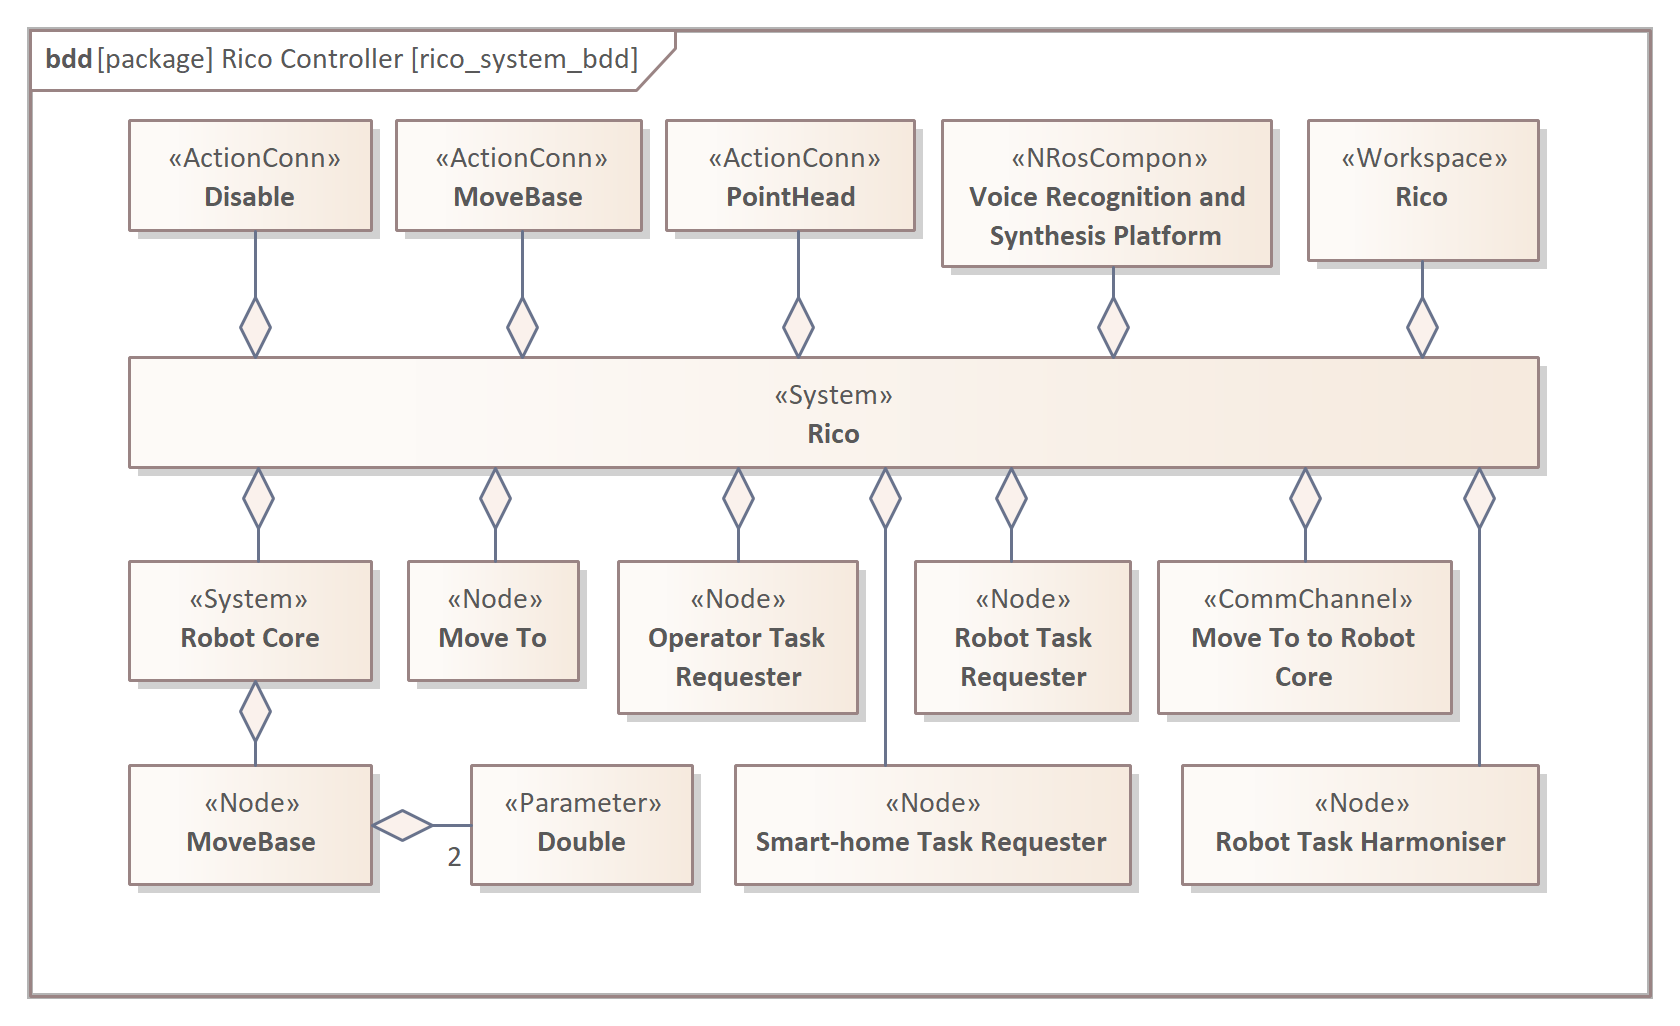
\includegraphics[scale=.9]{img/rico_pkg/rico_system_bdd.png}}
		\end{center}
		\caption{Rico \stSystem{} composition.} 
		\label{fig:rico_system_bdd}
	\end{figure}
	
	
	The fragment of the application scenario is conceptually presented in Fig.~\ref{fig:general_sd}.
	

	\begin{figure}[H] 
		\centering
		\begin{center}
			{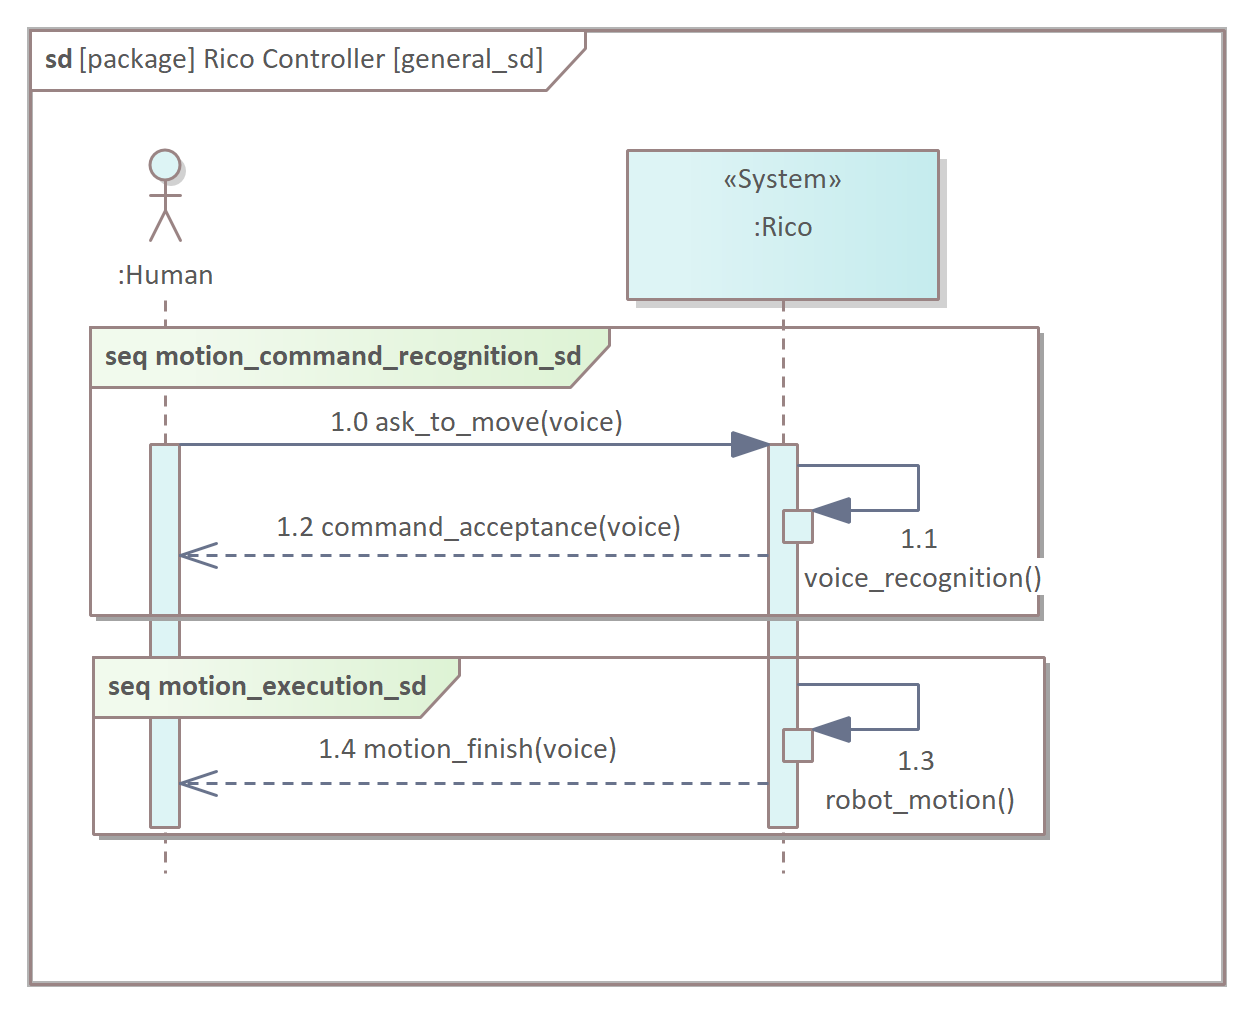
\includegraphics[scale=.9]{img/rico_pkg/general_sd.png}}
		\end{center}
		\caption{Concept scenario.} 
		\label{fig:general_sd}
	\end{figure}
	
	Here, the system (\stSystem{} \texttt{:Rico}) and its behaviour are formulated in a~general way. An actor (e.g. an elderly person) asks the robot to move. Then, the system recognises the voice command and vocally confirms the command's acceptance. Finally, the robot executes the motion and vocally informs that the motion is finished.
	In the following part of the description, the \stSystem{} \texttt{:Rico} and sequence diagram frame \texttt{motion execution} from Fig.~\ref{fig:general_sd} are presented in a~explicit way.
	
		The \stSystem{} \texttt{:Rico} structure is depicted in Fig.~\ref{fig:rico_system_ibd}. Here, and in the following diagrams, the \texttt{rosout} and \texttt{ROS master} \stNode{}s were omitted to make the diagrams more compact. Dedicated block is needed for \stCommChannel{} \texttt{:Move To to Robot Core}, because this \stCommChannel{} is specified in detail later on.
	
	\begin{figure}[H]
		\centering
		\begin{center}
			{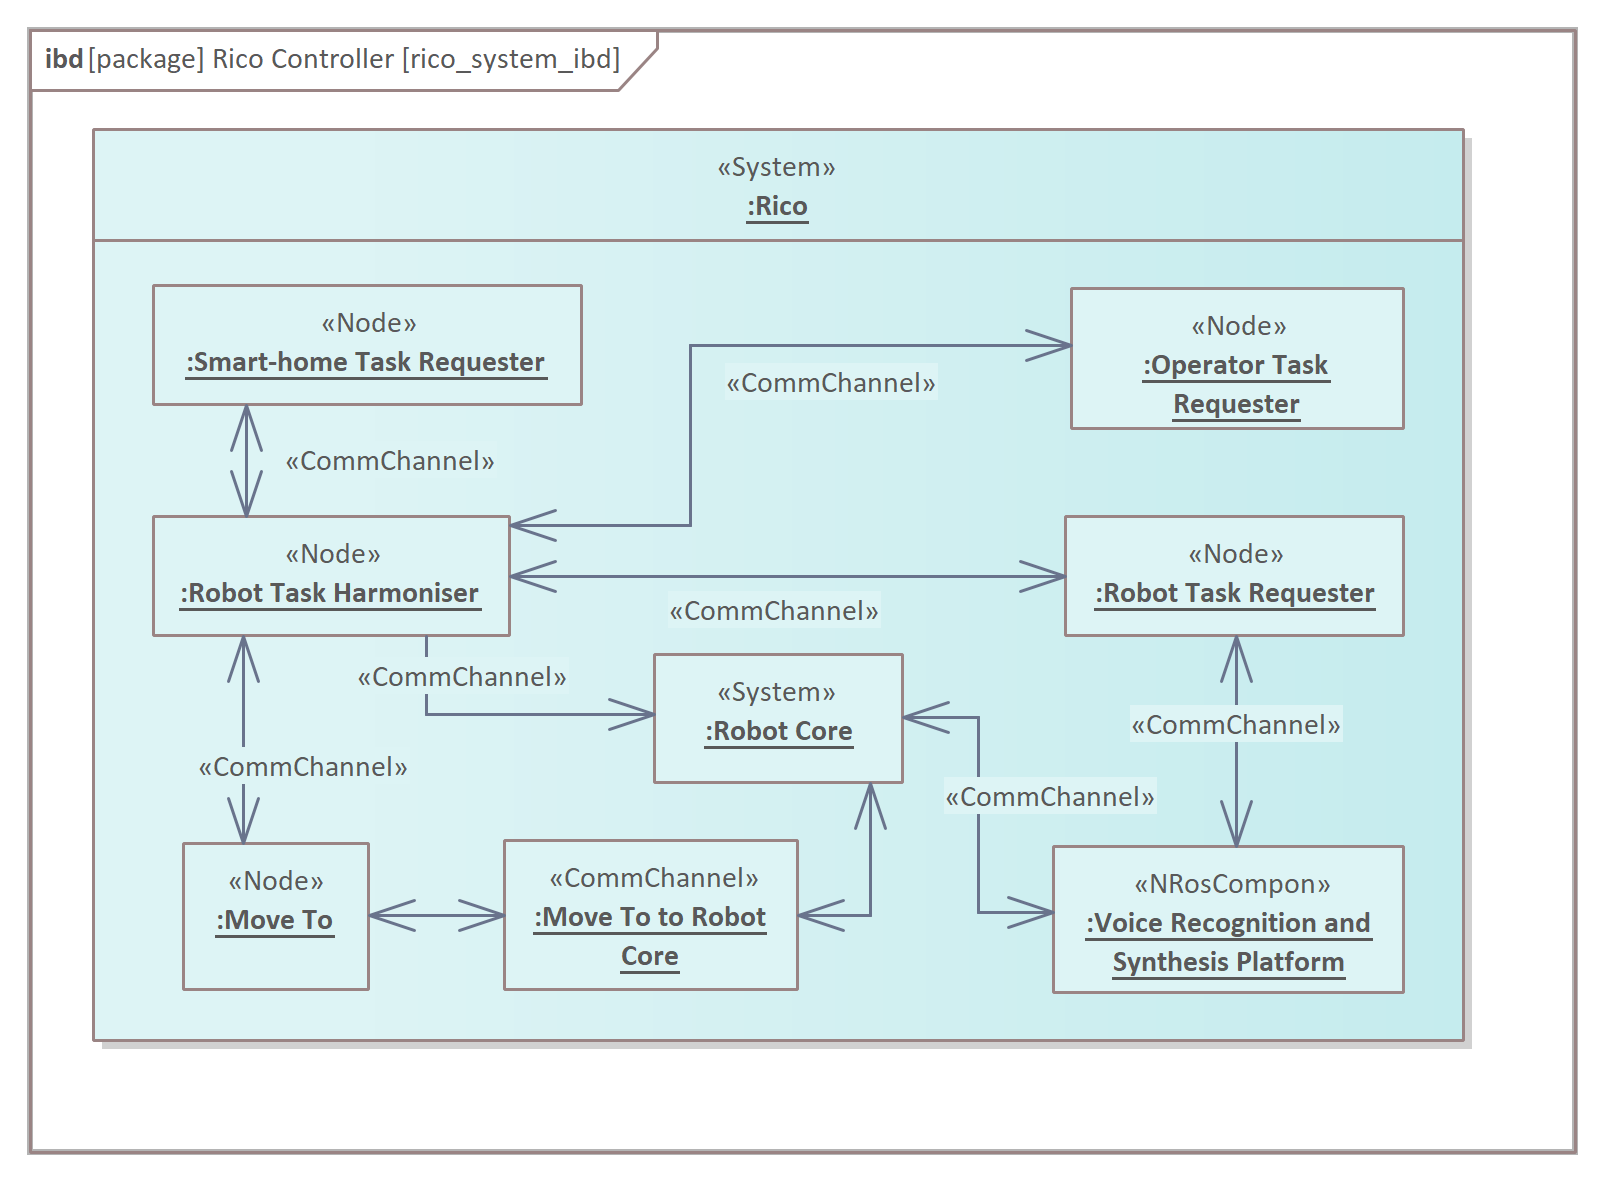
\includegraphics[scale=0.85]{img/rico_pkg/rico_system_ibd.png}}
		\end{center}
		\caption{Structure of \stSystem{}\texttt{:Rico}.} 
		\label{fig:rico_system_ibd}
	\end{figure}

	The system is based on TaskER framework \cite{tasker2020} developed from the RAPP approach to construct systems with variable structure \cite{zielinski2017variable}. The role of the TaskER is to schedule a~robot’s tasks. It consists of (i) Task Requesters \stNode{}s to submit new tasks, (ii) Task Harmoniser \stNode{} to schedule tasks execution, (iii) dynamic \stNode{}s (here, \stNode{} \texttt{:Move To}) to execute a~particular task on the robot hardware and (iv) cloud part, here <<NRosCompon>> \texttt{:Voice Recognition and Synthesis Platform}. The common part of the controller is located in \stSystem{} \texttt{:Rico}.
	
	Fig.~\ref{fig:robot_core_ibd} illustrates how various instances of the same block are depicted in the model. Two \stParameter{} Objects of the same classifier \texttt{:Double} are composed into \stNode{} \texttt{:MoveBase}.
	
	\begin{figure}[H]
		\centering
		\begin{center}
			{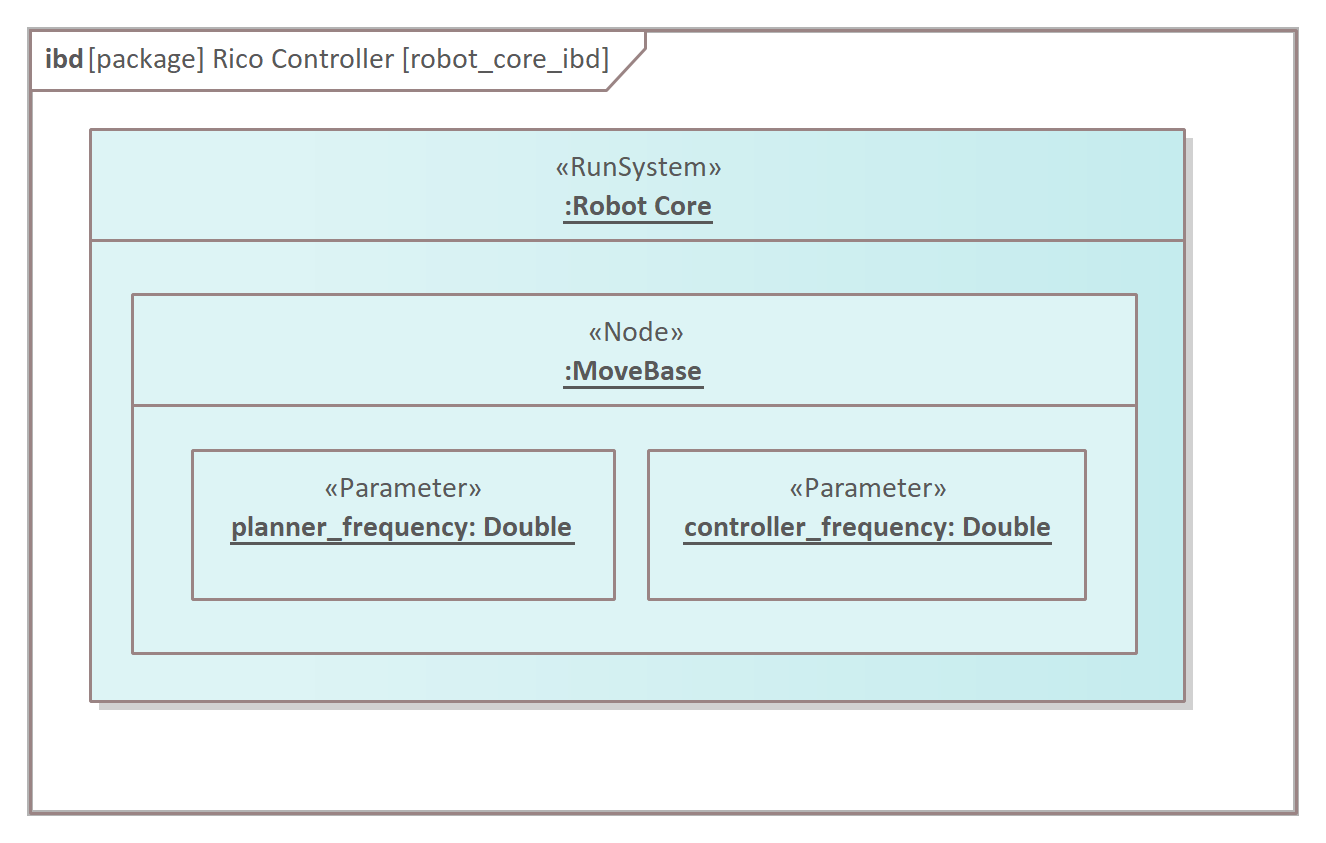
\includegraphics[scale=.85]{img/rico_pkg/robot_core_ibd.png}}
		\end{center}
		\caption{Selected elements of \stSystem{} \texttt{:Robot Core}.} 
		\label{fig:robot_core_ibd}
	\end{figure}
				
	\stCommChannel{} \texttt{:Move To to Robot Core} is depicted in Fig.~\ref{fig:move_to_2_core_cm_ibd}. It comprises three actions.
	

	\begin{figure}[H]
		\centering
		\begin{center}
			{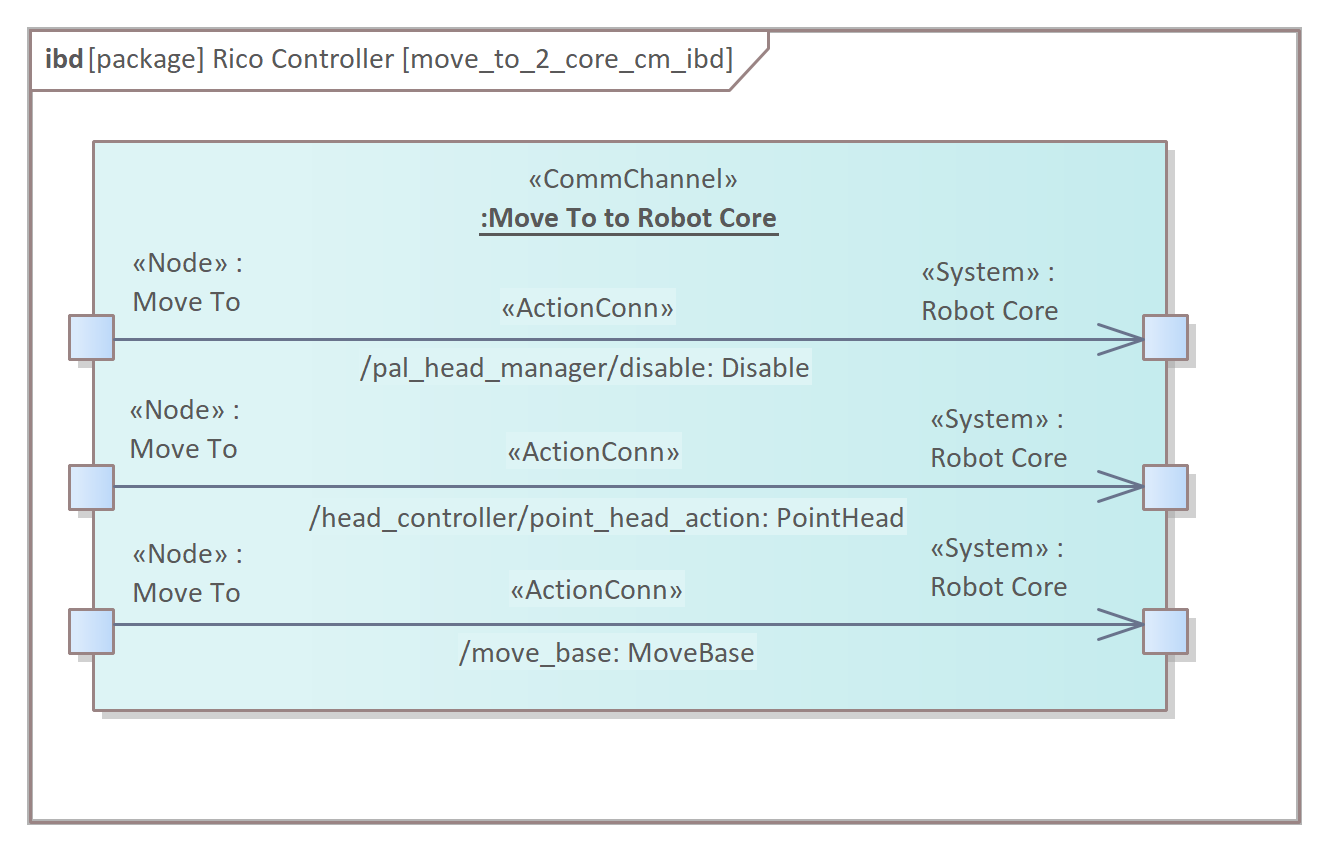
\includegraphics[scale=1.1]{img/rico_pkg/move_to_2_core_cm_ibd.png}}
		\end{center}
		\caption{Example of \stCommChannel{}.} 
		\label{fig:move_to_2_core_cm_ibd}
	\end{figure}
	
		
	The part of the scenario generally described in Fig.~\ref{fig:general_sd} is depicted in detail in Fig.~\ref{fig:motion_execution_sd}. The presentation remains conceptual from the behavioural point of view, but it considers the particular parts of the \stSystem{} \texttt{:Rico}.
	
	\begin{figure}[H]
		\centering
		\begin{center}
			{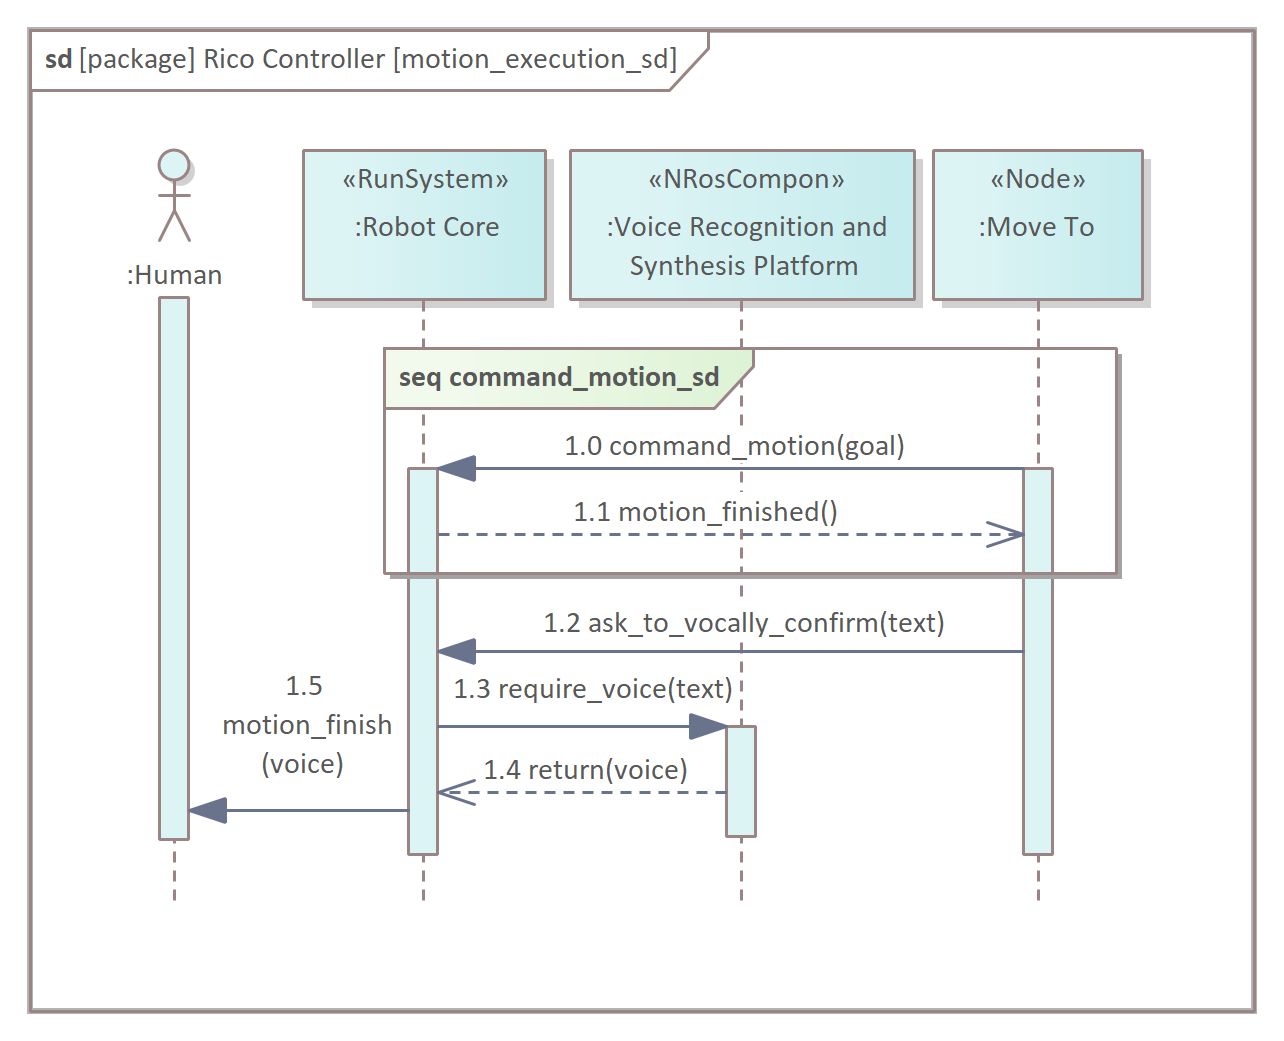
\includegraphics[scale=1.1]{img/rico_pkg/motion_execution_sd.png}}
		\end{center}
		\caption{Motion execution operation.} 
		\label{fig:motion_execution_sd}
	\end{figure}


	Finally, the particular communication methods are specified on the most detailed, ROS-specific level (Fig.~\ref{fig:command_motion_sd}). The command\_motion operation includes the sequence of four steps of communication. Three Actions realise the communication, one utilised twice. The diagram comprises extra notes that make it easier to interpret.
	
	\begin{figure}[H]
		\centering
		\begin{center}
			{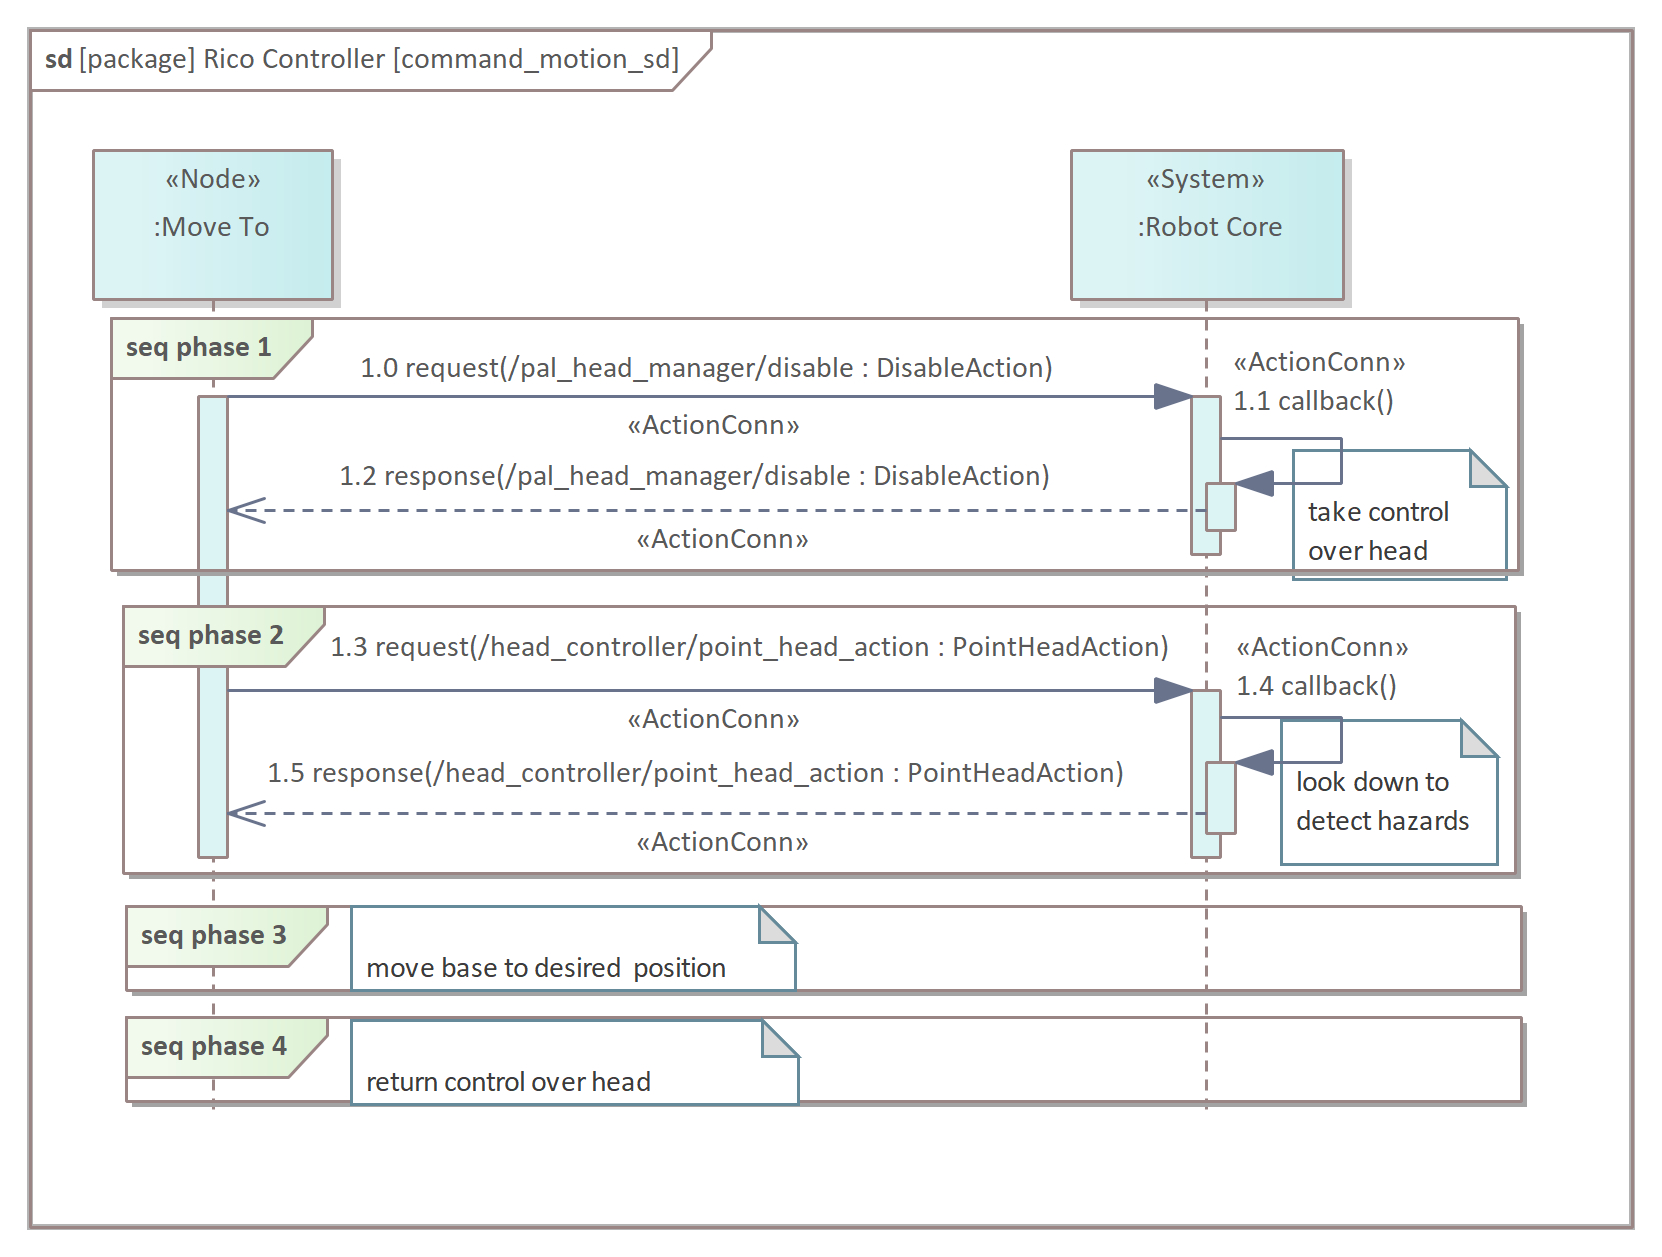
\includegraphics[scale=1.0]{img/rico_pkg/command_motion_sd.png}}
		\end{center}
		\caption{Command motion operation with detailed Communication methods presentation.} 
		\label{fig:command_motion_sd}
	\end{figure}
	
	The part of the \stWorkspace{} \texttt{:Rico} that includes previously mentioned elements is presented in Fig.~\ref{fig:rico_workspace_nodes_bdd} and Fig.~\ref{fig:rico_workspace_msgs_bdd}.
	
	\begin{figure}[H]
		\centering
		\begin{center}
			{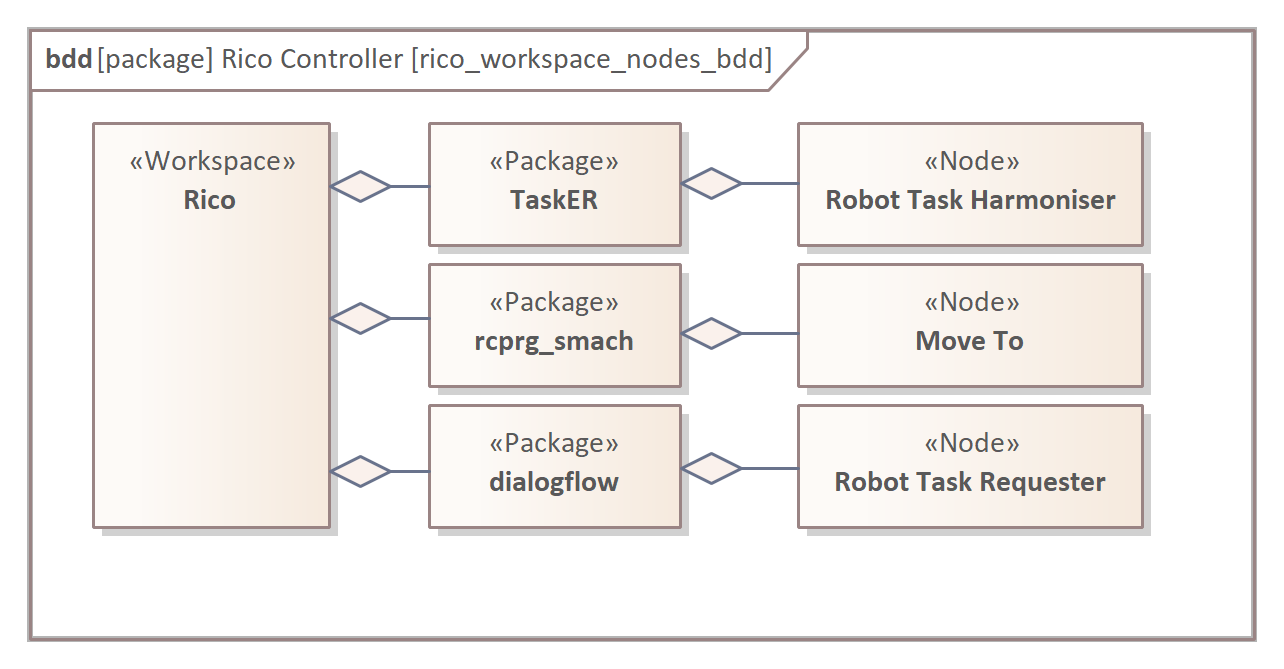
\includegraphics[scale=1.0]{img/rico_pkg/rico_workspace_nodes_bdd.png}}
		\end{center}
		\caption{Rico \stWorkspace{} composition -- Packages with Nodes.}
		\label{fig:rico_workspace_nodes_bdd}
	\end{figure}

	\begin{figure}[H]
		\centering
		\begin{center}
			{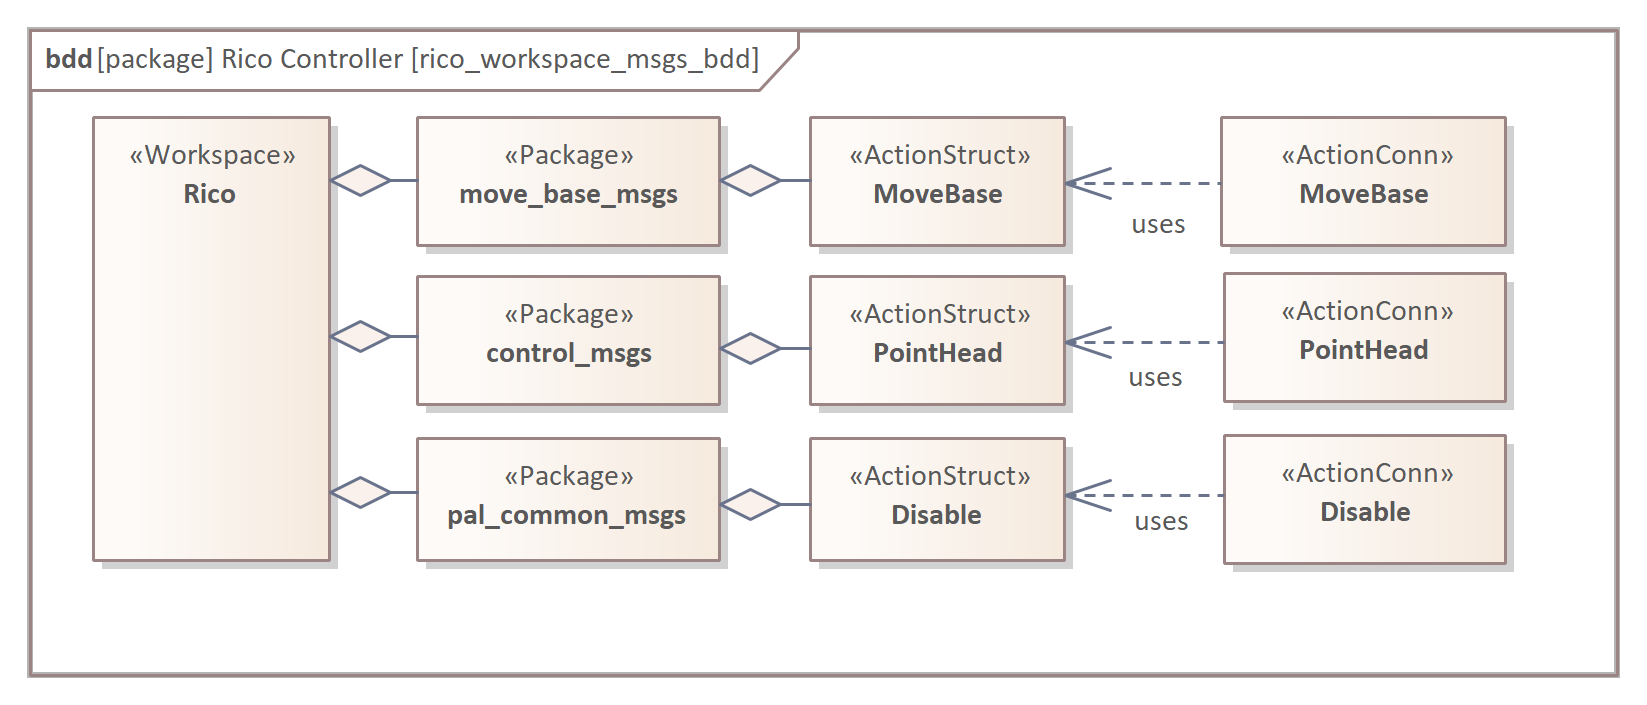
\includegraphics[scale=1.0]{img/rico_pkg/rico_workspace_msgs_bdd.png}}
		\end{center}
		\caption{Rico \stWorkspace{} composition -- Packages with Msgs.}
		\label{fig:rico_workspace_msgs_bdd}
	\end{figure}
	
			
\AtNextBibliography{\small}
\printbibliography
	
\end{document}
